\documentclass[a4paper]{scrartcl}

\usepackage[
	fancytheorems,
	fancyproofs,
	noindent
]{adam}

\usepackage{tikz}
\usepackage{mathtools}

\newcommand{\QQ}{\mathbb{Q}}
\newcommand{\dP}{\mathrm{d}\PP}
\newcommand{\dQ}{\mathrm{d}\QQ}
\newcommand{\sd}{\operatorname{sd}}

\title{Stochastic Financial Models}
\author{Adam Kelly (\texttt{ak2316@cam.ac.uk})}
\date{\today}

\allowdisplaybreaks

\begin{document}

\maketitle

Financial markets are, from a mathematician's point of view, a rather remarkable object of study. They are made of people, and people are not easy to axiomatise. And yet if we grant ourselves a single principle -- that one cannot make something out of nothing -- then a startling amount of structure falls out. Prices of complicated derivative securities are pinned down exactly by the prices of simple ones; the `right' probability measure to compute with turns out not to be the one describing what will actually happen; and the whole edifice rests on the theory of martingales.

This course is really two courses braided together. One strand is economic: how should an agent with preferences choose a portfolio, and what does market equilibrium look like? The other strand is probabilistic: conditional expectation, martingales, optional stopping, Brownian motion, and a first look at stochastic calculus. The two strands meet in the \emph{fundamental theorem of asset pricing}, which says that a market admits no arbitrage precisely when there is an equivalent measure making discounted prices into martingales. Everything after that theorem is, in one way or another, a computation of a conditional expectation.

This article constitutes my notes for the `Stochastic Financial Models' course, held in Michaelmas 2021 at Cambridge. These notes are \emph{not a transcription of the lectures}, and differ significantly in quite a few areas. Still, all lectured material should be covered.

\tableofcontents

\clearpage

\section{The One-Period Market}

Before we can prove anything, we need a model. The models in this course are deliberately, almost offensively, simple; the justification is that even the simplest of them already produces the Black--Scholes formula, and that the qualitative conclusions turn out to be robust.

\subsection{Standing Assumptions}

We shall work throughout under the following idealisations, which we state once and then quietly forget.

\begin{enumerate}[label=(\roman*)]
	\item \emph{No transaction costs.} Buying and selling are free.
	\item \emph{Infinite divisibility.} We may hold any real number of units of any asset, not just an integer number.
	\item \emph{No bid--ask spread.} There is one price at which an asset may be both bought and sold.
	\item \emph{No price impact} (`linear pricing'). Buying $2\theta$ units costs exactly twice as much as buying $\theta$ units, however large $\theta$ is. Our trading does not move the market.
	\item \emph{No short-selling constraints.} We may hold a negative number of units of an asset.
	\item \emph{Borrowing and lending at the same rate.} There is a riskless bank account paying interest at rate $r$, and we may deposit into it or borrow from it freely.
\end{enumerate}

Assumption (iv) is the one doing the most work, and it is also the one most obviously false: if you try to buy every share in a company you will find the price moves against you. But without it there is no hope of a linear theory, and linearity is what makes everything computable.

\subsection{Portfolios and Wealth}

Our basic market has $d$ \vocab{risky assets}, whose prices at time $t$ we write as a random vector
$$
S_t = (S_t^1, \dots, S_t^d)^\top.
$$
For the moment there are only two times, $t = 0$ and $t = 1$; this is the \vocab{one-period model}. The price $S_0$ is known at time $0$, and $S_1$ is a random vector whose distribution we assume known. In addition there is a \vocab{riskless asset} (asset $0$, the bank account) which turns one pound at time $0$ into $1 + r$ pounds at time $1$.

\begin{definition}[Portfolio]
	A \vocab{portfolio} is a vector $\theta = (\theta^1, \dots, \theta^d)^\top \in \R^d$, where $\theta^i$ is the number of units of asset $i$ held between time $0$ and time $1$, together with a number $\theta^0 \in \R$ of pounds in the bank.
\end{definition}

If $\theta^i > 0$ we say the agent is \vocab{long} asset $i$; if $\theta^i < 0$ the agent is \vocab{short} it, meaning that they have borrowed the asset and sold it, and must return it at time $1$.

Let $X_t$ denote the agent's wealth at time $t$, with $X_0 = x$ given. Since the portfolio must be paid for out of the initial wealth, we have the \vocab{budget constraint}
$$
X_0 = \theta^0 + \theta^\top S_0.
$$
At time $1$ the bank deposit has grown and the shares are worth $\theta^\top S_1$, so
$$
X_1 = \theta^0(1+r) + \theta^\top S_1 = (1+r)\left(X_0 - \theta^\top S_0\right) + \theta^\top S_1.
$$
Rearranging gives an expression which will be with us for the rest of the course:
$$
\boxed{\;X_1 = (1+r)X_0 + \theta^\top\big(S_1 - (1+r)S_0\big).\;}
$$
In other words -- the wealth at time $1$ is what you would have got by leaving everything in the bank, plus a term measuring how much better the risky assets did than the bank. We give that term a name.

\begin{definition}[Excess return]
	The \vocab{excess return vector} of the market is
	$$
	\xi = S_1 - (1+r)S_0 \in \R^d.
	$$
\end{definition}

So $X_1 = (1+r)X_0 + \theta^\top \xi$, and the whole of the one-period theory is really the study of the random vector $\xi$. Note that $\xi$ is genuinely random -- it is the only randomness in the model -- and that the map $\theta \mapsto \theta^\top \xi$ is linear. Almost every theorem below is a statement about the linear subspace $\{\theta^\top \xi : \theta \in \R^d\}$ of random variables.

We write $\mathcal{X}(x) = \{(1+r)x + \theta^\top \xi : \theta \in \R^d\}$ for the set of \vocab{attainable} time-$1$ wealths starting from initial wealth $x$. This is an affine subspace of the space of random variables.

\begin{remark}
	It is worth pausing to note what has \emph{not} been assumed. We have not assumed that the agent knows anything about $S_1$ beyond its distribution, and we have certainly not assumed that this distribution is correct. Estimating it is a large industry (and something you might recognise from Part IB Statistics); it is not our concern here.
\end{remark}

\subsection{A First Example}

Let us immediately do a computation, so that the abstractions have something to hang on.

\begin{example}[A one-period binomial market]
	Take $d = 1$, interest rate $r = 0$, and $S_0 = 5$. Suppose $S_1$ takes the value $7$ or the value $4$, each with probability $\tfrac12$. Consider a \vocab{call option} with strike $K = 6$: this is the right, but not the obligation, to buy one share at time $1$ for the price $6$. If $S_1 = 7$ we exercise the right and make $1$; if $S_1 = 4$ we do not, and make $0$. So the payout is
	$$
	Y = (S_1 - K)^+ = \begin{cases} 1 & \text{if } S_1 = 7,\\ 0 & \text{if } S_1 = 4.\end{cases}
	$$
	What is this option worth at time $0$? A first guess might be $\EE Y = \tfrac12$. That guess is wrong, and the reason it is wrong is the whole point of the course.

	Observe that $Y = \tfrac13(S_1 - 4)$: indeed $\tfrac13(7-4) = 1$ and $\tfrac13(4-4) = 0$. So if at time $0$ we buy $\tfrac13$ of a share and borrow $\tfrac43$ from the bank, our time-$1$ wealth is exactly $\tfrac13 S_1 - \tfrac43 = Y$, whatever happens. The cost of setting this up is
	$$
	\tfrac13 \cdot 5 - \tfrac43 = \tfrac53 - \tfrac43 = \tfrac13.
	$$
	So a portfolio costing $\tfrac13$ reproduces the option payout exactly. If the option were sold for more than $\tfrac13$, we could sell the option, set up the portfolio, and pocket the difference with no risk whatsoever; if it were sold for less, we would do the reverse. So the only price consistent with the absence of a free lunch is $\tfrac13$.

	There is a second route to the same number. Suppose we pretend the probability of the up-move is $q$ rather than $\tfrac12$, chosen so that the share price is `fair', i.e.\ $\EE_{\QQ}[S_1] = (1+r)S_0 = 5$. Then $7q + 4(1-q) = 5$, giving $q = \tfrac13$. And under this measure,
	$$
	\frac{\EE_\QQ[Y]}{1+r} = \tfrac13 \cdot 1 + \tfrac23 \cdot 0 = \tfrac13.
	$$
	The same answer. That this is not a coincidence is the content of the fundamental theorem of asset pricing, which we prove in \S4.
\end{example}

Notice that the true probability $p = \tfrac12$ played no role at all in the answer. This is the single most counterintuitive feature of derivative pricing, and it is worth being clear about why it happens: the option payout is a \emph{deterministic function} of the share price, and the share price is already trading at a known price. All the information about probabilities that we need is already baked into $S_0 = 5$.

\section{Mean-Variance Analysis}

Our agent has to choose a portfolio $\theta$. On what basis? The oldest quantitative answer, due to Markowitz in 1952, is: get the expected return you want, and take as little risk as possible along the way, where `risk' means variance.

\subsection{The Markowitz Problem}

\begin{definition}[Mean-variance portfolio problem]
	Given initial wealth $X_0 = x$ and a target mean $m \in \R$, the \vocab{mean-variance portfolio problem} is to
	$$
	\text{minimise } \var(X_1) \quad \text{subject to} \quad \EE[X_1] = m,
	$$
	over portfolios $\theta \in \R^d$.
\end{definition}

Throughout this section we assume that $S_1$ is square integrable, and we write
$$
\mu = \EE[S_1], \qquad V = \cov(S_1) = \EE\big[(S_1 - \mu)(S_1-\mu)^\top\big].
$$
The matrix $V$ is always non-negative definite; we assume in addition that it is \emph{positive} definite, so that $V^{-1}$ exists. (If it is not, some portfolio of the risky assets is riskless, and one should first remove the redundancy.) We also assume $\mu \neq (1+r)S_0$, since otherwise the risky assets offer no expected reward over the bank and the problem is uninteresting.

Since $X_1 = (1+r)x + \theta^\top \xi$ with $\xi = S_1 - (1+r)S_0$, we have
$$
\EE[X_1] = (1+r)x + \theta^\top(\mu - (1+r)S_0), \qquad \var(X_1) = \theta^\top V \theta.
$$
So the problem is: minimise the quadratic form $\theta^\top V\theta$ subject to the affine constraint $\theta^\top(\mu - (1+r)S_0) = m - (1+r)x$. This is a problem you could do with Lagrange multipliers, but there is a slicker argument which also delivers uniqueness for free.

\begin{theorem}[Markowitz]\label{thm:markowitz}
	Write $\nu = \mu - (1+r)S_0$. The mean-variance portfolio problem has the unique solution
	$$
	\theta^* = \lambda V^{-1}\nu, \qquad \lambda = \frac{m - (1+r)x}{\nu^\top V^{-1}\nu}.
	$$
\end{theorem}

\begin{proof}
	First, $\theta^*$ is feasible: $(\theta^*)^\top \nu = \lambda \nu^\top V^{-1}\nu = m - (1+r)x$, as required.

	Now let $\theta$ be any other feasible portfolio and set $\epsilon = \theta - \theta^* \neq 0$. Expanding,
	$$
	\theta^\top V \theta = (\theta^*)^\top V \theta^* + 2\epsilon^\top V \theta^* + \epsilon^\top V \epsilon.
	$$
	The cross term vanishes: since both $\theta$ and $\theta^*$ are feasible, $\epsilon^\top \nu = 0$, and hence
	$$
	\epsilon^\top V \theta^* = \lambda\, \epsilon^\top V V^{-1}\nu = \lambda\, \epsilon^\top \nu = 0.
	$$
	As $V$ is positive definite and $\epsilon \neq 0$ we get $\epsilon^\top V\epsilon > 0$, so $\theta^\top V\theta > (\theta^*)^\top V\theta^*$. Hence $\theta^*$ is the unique minimiser.
\end{proof}

The vector $V^{-1}\nu$ appearing here is important enough to be named.

\begin{definition}[Market portfolio]
	The \vocab{market portfolio} is $\theta^{\mathrm{mar}} = V^{-1}\big(\mu - (1+r)S_0\big)$, and we write $S_t^{\mathrm{mar}} = (\theta^{\mathrm{mar}})^\top S_t$ for its price.
\end{definition}

\begin{corollary}[Mutual fund theorem]
	A portfolio is mean-variance efficient if and only if it is a scalar multiple of the market portfolio.
\end{corollary}

\begin{proof}
	Immediate from Theorem~\ref{thm:markowitz}: the optimal $\theta^*$ is $\lambda \theta^{\mathrm{mar}}$, and as $m$ ranges over $\R$, $\lambda$ ranges over $\R$.
\end{proof}

This is a genuinely striking conclusion. Every investor, no matter how risk-hungry or risk-shy, should hold the risky assets \emph{in the same proportions}; the only thing that distinguishes them is how much they put in the bank. In practice this is the theoretical justification for index funds: if the theory holds, you need exactly two products, a bank account and one fund.

\subsection{The Efficient Frontier}

As $\theta$ ranges over $\R^d$, the pair $(\var(X_1), \EE[X_1])$ traces out a subset of the right half plane. Its left-hand boundary is the object of interest.

\begin{definition}[Efficient frontier]
	The \vocab{mean-variance efficient frontier} is the set of points
	$$
	\left\{ \big(\min\{\var(X_1) : \EE[X_1] = m\},\, m\big) : m \in \R \right\}.
	$$
	A portfolio achieving a point of the frontier is called \vocab{mean-variance efficient}.
\end{definition}

\begin{corollary}[Shape of the frontier]\label{cor:frontier}
	In the $(v,m)$ plane the efficient frontier is the parabola
	$$
	v = \frac{\big(m - (1+r)x\big)^2}{\nu^\top V^{-1}\nu}, \qquad \nu = \mu - (1+r)S_0.
	$$
\end{corollary}

\begin{proof}
	Substituting $\theta^* = \lambda V^{-1}\nu$ into $v = \theta^\top V\theta$ gives $v = \lambda^2 \nu^\top V^{-1}\nu$, and $\lambda = (m - (1+r)x)/(\nu^\top V^{-1}\nu)$.
\end{proof}

It is more usual, and more informative, to plot the frontier in the $(\sigma, m)$ plane, where $\sigma = \sd(X_1) = \sqrt{v}$ is the standard deviation. Taking square roots in Corollary~\ref{cor:frontier}, the frontier becomes a pair of \emph{straight lines} through the point $(0, (1+r)x)$, of slopes $\pm\sqrt{\nu^\top V^{-1}\nu}$. Only the upper line is of any interest -- given a level of risk one wants the larger mean -- and it is called the \vocab{capital market line}. Its slope
$$
\frac{m - (1+r)x}{\sigma} = \sqrt{\nu^\top V^{-1}\nu}
$$
is the \vocab{Sharpe ratio}, the amount of excess expected return purchased per unit of risk.

If we forbid the agent from using the bank account, and force them to hold only risky assets, then the corresponding frontier is instead a hyperbola in the $(\sigma,m)$ plane, with a leftmost point (the \vocab{minimum-variance portfolio}). The capital market line is tangent to that hyperbola, and the point of tangency is exactly the market portfolio, normalised to cost $x$. The picture to hold in your head is the following.

\begin{center}
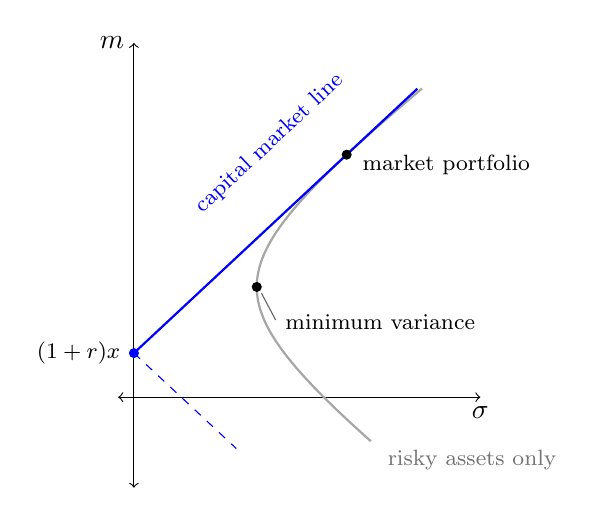
\begin{tikzpicture}[scale=1.0]
	\draw[<->] (-0.2,0) -- (4.4,0) node[below] {$\sigma$};
	\draw[<->] (0,-1.15) -- (0,4.5) node[left] {$m$};
	% risky-only frontier (hyperbola)
	\draw[thick, color=black!35]
    (3.0097,-0.5600) -- (2.9783,-0.5320) -- (2.9471,-0.5040) -- (2.9159,-0.4760) -- (2.8849,-0.4480) -- (2.8541,-0.4200) --
    (2.8234,-0.3920) -- (2.7928,-0.3640) -- (2.7624,-0.3360) -- (2.7321,-0.3080) -- (2.7020,-0.2800) -- (2.6721,-0.2520) --
    (2.6423,-0.2240) -- (2.6127,-0.1960) -- (2.5833,-0.1680) -- (2.5541,-0.1400) -- (2.5251,-0.1120) -- (2.4963,-0.0840) --
    (2.4677,-0.0560) -- (2.4393,-0.0280) -- (2.4111,0.0000) -- (2.3832,0.0280) -- (2.3555,0.0560) -- (2.3281,0.0840) --
    (2.3010,0.1120) -- (2.2741,0.1400) -- (2.2475,0.1680) -- (2.2211,0.1960) -- (2.1951,0.2240) -- (2.1694,0.2520) --
    (2.1440,0.2800) -- (2.1190,0.3080) -- (2.0943,0.3360) -- (2.0699,0.3640) -- (2.0459,0.3920) -- (2.0223,0.4200) --
    (1.9991,0.4480) -- (1.9763,0.4760) -- (1.9540,0.5040) -- (1.9321,0.5320) -- (1.9106,0.5600) -- (1.8896,0.5880) --
    (1.8691,0.6160) -- (1.8491,0.6440) -- (1.8296,0.6720) -- (1.8107,0.7000) -- (1.7923,0.7280) -- (1.7745,0.7560) --
    (1.7573,0.7840) -- (1.7406,0.8120) -- (1.7246,0.8400) -- (1.7093,0.8680) -- (1.6946,0.8960) -- (1.6806,0.9240) --
    (1.6672,0.9520) -- (1.6546,0.9800) -- (1.6427,1.0080) -- (1.6316,1.0360) -- (1.6212,1.0640) -- (1.6116,1.0920) --
    (1.6027,1.1200) -- (1.5947,1.1480) -- (1.5875,1.1760) -- (1.5811,1.2040) -- (1.5755,1.2320) -- (1.5708,1.2600) --
    (1.5669,1.2880) -- (1.5639,1.3160) -- (1.5617,1.3440) -- (1.5604,1.3720) -- (1.5600,1.4000) -- (1.5604,1.4280) --
    (1.5617,1.4560) -- (1.5639,1.4840) -- (1.5669,1.5120) -- (1.5708,1.5400) -- (1.5755,1.5680) -- (1.5811,1.5960) --
    (1.5875,1.6240) -- (1.5947,1.6520) -- (1.6027,1.6800) -- (1.6116,1.7080) -- (1.6212,1.7360) -- (1.6316,1.7640) --
    (1.6427,1.7920) -- (1.6546,1.8200) -- (1.6672,1.8480) -- (1.6806,1.8760) -- (1.6946,1.9040) -- (1.7093,1.9320) --
    (1.7246,1.9600) -- (1.7406,1.9880) -- (1.7573,2.0160) -- (1.7745,2.0440) -- (1.7923,2.0720) -- (1.8107,2.1000) --
    (1.8296,2.1280) -- (1.8491,2.1560) -- (1.8691,2.1840) -- (1.8896,2.2120) -- (1.9106,2.2400) -- (1.9321,2.2680) --
    (1.9540,2.2960) -- (1.9763,2.3240) -- (1.9991,2.3520) -- (2.0223,2.3800) -- (2.0459,2.4080) -- (2.0699,2.4360) --
    (2.0943,2.4640) -- (2.1190,2.4920) -- (2.1440,2.5200) -- (2.1694,2.5480) -- (2.1951,2.5760) -- (2.2211,2.6040) --
    (2.2475,2.6320) -- (2.2741,2.6600) -- (2.3010,2.6880) -- (2.3281,2.7160) -- (2.3555,2.7440) -- (2.3832,2.7720) --
    (2.4111,2.8000) -- (2.4393,2.8280) -- (2.4677,2.8560) -- (2.4963,2.8840) -- (2.5251,2.9120) -- (2.5541,2.9400) --
    (2.5833,2.9680) -- (2.6127,2.9960) -- (2.6423,3.0240) -- (2.6721,3.0520) -- (2.7020,3.0800) -- (2.7321,3.1080) --
    (2.7624,3.1360) -- (2.7928,3.1640) -- (2.8234,3.1920) -- (2.8541,3.2200) -- (2.8849,3.2480) -- (2.9159,3.2760) --
    (2.9471,3.3040) -- (2.9783,3.3320) -- (3.0097,3.3600) -- (3.0412,3.3880) -- (3.0728,3.4160) -- (3.1046,3.4440) --
    (3.1364,3.4720) -- (3.1684,3.5000) -- (3.2004,3.5280) -- (3.2326,3.5560) -- (3.2648,3.5840) -- (3.2972,3.6120) --
    (3.3296,3.6400) -- (3.3622,3.6680) -- (3.3948,3.6960) -- (3.4275,3.7240) -- (3.4602,3.7520) -- (3.4931,3.7800) --
    (3.5260,3.8080) -- (3.5591,3.8360) -- (3.5921,3.8640) -- (3.6253,3.8920) -- (3.6585,3.9200)
	;
	% capital market line
	\draw[thick, color=blue] (0,0.56) -- (3.6,3.918);
	\draw[dashed, color=blue] (0,0.56) -- (1.3,-0.652);
	\filldraw[color=blue] (0,0.56) circle (1.6pt);
	\node[left] at (-0.05,0.56) {\footnotesize $(1+r)x$};
	\filldraw[color=black] (2.702,3.08) circle (1.6pt);
	\node[right] at (2.78,2.95) {\footnotesize market portfolio};
	\filldraw[color=black] (1.56,1.40) circle (1.6pt);
	\draw[thin, color=black!60] (1.62,1.32) -- (1.80,0.98);
	\node[right] at (1.80,0.95) {\footnotesize minimum variance};
	\node[color=blue, rotate=43] at (1.72,3.22) {\footnotesize capital market line};
	\node[color=black!55, right] at (3.10,-0.80) {\footnotesize risky assets only};
\end{tikzpicture}
\end{center}

The dashed part of the capital market line corresponds to $\lambda < 0$, i.e.\ to shorting the market portfolio; those portfolios solve the minimisation problem but no sensible agent would choose them.

\begin{corollary}
	The problem of minimising $\var(X_1)$ subject to $\EE[X_1] \geq m$ has the same solution as the mean-variance problem whenever $m \geq (1+r)x$. If $m < (1+r)x$, the solution is $\theta = 0$.
\end{corollary}

\begin{proof}
	If $m \geq (1+r)x$ then the constraint binds, since variance is increasing in $|\lambda|$ and the mean is increasing in $\lambda$. If $m < (1+r)x$ then $\theta = 0$ gives $\var(X_1) = 0$ and $\EE[X_1] = (1+r)x \geq m$, which is clearly optimal.
\end{proof}

\begin{remark}
	Variance is a strange measure of risk. It punishes unexpectedly \emph{good} outcomes exactly as much as unexpectedly bad ones, and it takes no account of the shape of the tail. We will replace it with something better in \S3. On the other hand, mean-variance analysis has the enormous advantage of being solvable in closed form, which is why it is still used.
\end{remark}

\subsection{The Capital Asset Pricing Model}

We now ask an equilibrium question: if \emph{everyone} behaves as in the previous section, what do prices look like? The answer is the capital asset pricing model of Sharpe (1964), and its content is that the expected excess return of any asset is determined by a single number, its exposure to the market as a whole.

We begin with an entirely elementary fact, which is just linear regression.

\begin{proposition}\label{prop:regression}
	Let $X, Y$ be square integrable random variables with $\var(X) > 0$. Then there are unique constants $\alpha, \beta$ such that
	$$
	Y = \alpha + \beta X + Z, \qquad \EE[Z] = 0, \quad \cov(Z,X) = 0.
	$$
	Explicitly, $\beta = \cov(X,Y)/\var(X)$ and $\alpha = \EE[Y] - \beta\,\EE[X]$.
\end{proposition}

\begin{proof}
	Setting $Z = Y - \alpha - \beta X$, the two conditions read
	$$
	0 = \EE[Y] - \alpha - \beta \EE[X], \qquad 0 = \cov(Y,X) - \beta\var(X),
	$$
	which have the unique solution stated.
\end{proof}

Now let us specialise to the market portfolio. Recall $S^{\mathrm{mar}}_t = (\theta^{\mathrm{mar}})^\top S_t$ and write $\xi = S_1 - (1+r)S_0$, $\xi^{\mathrm{mar}} = S_1^{\mathrm{mar}} - (1+r)S_0^{\mathrm{mar}} = (\theta^{\mathrm{mar}})^\top \xi$.

\begin{theorem}\label{thm:capm-vector}
	Let $B = \cov(S_1, S_1^{\mathrm{mar}})/\var(S_1^{\mathrm{mar}}) \in \R^d$ and set $Z = \xi - B\,\xi^{\mathrm{mar}}$. Then $\EE[Z] = 0$ and $\cov(Z, S_1^{\mathrm{mar}}) = 0$.
\end{theorem}

\begin{proof}
	Write $\nu = \mu - (1+r)S_0 = \EE[\xi]$, so $\theta^{\mathrm{mar}} = V^{-1}\nu$. Then
	$$
	\EE[\xi^{\mathrm{mar}}] = (\theta^{\mathrm{mar}})^\top \nu = \nu^\top V^{-1}\nu = (\theta^{\mathrm{mar}})^\top V \theta^{\mathrm{mar}} = \var(S_1^{\mathrm{mar}}),
	$$
	using $V\theta^{\mathrm{mar}} = \nu$. On the other hand
	$$
	\cov(S_1, S_1^{\mathrm{mar}}) = \cov(S_1,S_1)\theta^{\mathrm{mar}} = V V^{-1}\nu = \nu = \EE[\xi].
	$$
	Therefore $B = \EE[\xi]/\EE[\xi^{\mathrm{mar}}]$, whence $\EE[Z] = \EE[\xi] - B\,\EE[\xi^{\mathrm{mar}}] = 0$. Similarly,
	$$
	\cov(Z, S_1^{\mathrm{mar}}) = \cov(S_1,S_1^{\mathrm{mar}}) - B\var(S_1^{\mathrm{mar}}) = \nu - \nu = 0. \qedhere
	$$
\end{proof}

To turn this into an economic statement we need the market to clear. Suppose asset $i$ exists in total supply $n^i$, write $n = (n^1,\dots,n^d)^\top$, and define the \vocab{index return}
$$
R^{\mathrm{index}} = \frac{n^\top S_1}{n^\top S_0} - 1,
$$
the return on holding the entire market in proportion to supply. Let $R^i = S_1^i/S_0^i - 1$ be the return on asset $i$.

\begin{axiom}[CAPM assumptions]
	There are $K$ investors, with portfolios $\theta^1, \dots, \theta^K$ satisfying \vocab{market clearing} $\sum_{k} \theta^k = n$. Every investor agrees on the values of $\mu = \EE[S_1]$ and $V = \cov(S_1)$ (\emph{uniform beliefs}) and every investor holds a mean-variance efficient portfolio, though possibly with different target means (\emph{uniform preferences}).
\end{axiom}

\begin{theorem}[Capital asset pricing model]
	Under the above assumptions, write the regression
	$$
	R^i - r = \alpha^i + \beta^i\big(R^{\mathrm{index}} - r\big) + \epsilon^i, \qquad \EE[\epsilon^i]=0,\ \cov(R^{\mathrm{index}},\epsilon^i) = 0,
	$$
	as in Proposition~\ref{prop:regression}. Then $\alpha^i = 0$ for every $i$.
\end{theorem}

\begin{proof}
	By the mutual fund theorem each investor's portfolio is $\theta^k = \lambda_k \theta^{\mathrm{mar}}$ for some $\lambda_k \in \R$. Market clearing gives $n = \big(\sum_k \lambda_k\big)\theta^{\mathrm{mar}}$, so $n$ is a positive multiple of the market portfolio, and therefore
	$$
	R^{\mathrm{index}} = \frac{n^\top S_1}{n^\top S_0} - 1 = \frac{S_1^{\mathrm{mar}}}{S_0^{\mathrm{mar}}} - 1.
	$$
	Now apply Theorem~\ref{thm:capm-vector} coordinatewise. Dividing $\xi^i = B^i \xi^{\mathrm{mar}} + Z^i$ by $S_0^i$,
	$$
	R^i - r = \frac{1}{S_0^i}\big(S_1^i - (1+r)S_0^i\big) = \frac{B^i S_0^{\mathrm{mar}}}{S_0^i}\big(R^{\mathrm{index}} - r\big) + \frac{Z^i}{S_0^i}.
	$$
	Since $\EE[Z^i] = 0$ and $\cov(Z^i, R^{\mathrm{index}}) = 0$, uniqueness in Proposition~\ref{prop:regression} identifies $\beta^i = B^iS_0^{\mathrm{mar}}/S_0^i$, $\epsilon^i = Z^i/S_0^i$ and $\alpha^i = 0$.
\end{proof}

So under CAPM the expected excess return on asset $i$ is
$$
\EE[R^i] - r = \beta^i\big(\EE[R^{\mathrm{index}}] - r\big),
$$
and nothing else about asset $i$ matters. The quantity $\beta^i$ is a genuinely used piece of market vocabulary. An asset with $\beta = 1.5$ tends to move one and a half times as much as the market; an asset with $\beta = 0$ is uncorrelated with the market and, however volatile it may be on its own, commands no excess return at all, because its risk can be diversified away.

\begin{remark}
	It is worth being honest about the assumptions. Uniform beliefs is not plausible: if everyone agreed on $\mu$ and $V$ there would be very little trading. Uniform preferences is worse: we have already noted that variance is a poor proxy for risk. And empirically, when one regresses returns against the index, the estimated $\alpha$'s are not zero -- searching for assets with positive $\alpha$ is more or less the definition of active management. Nonetheless CAPM is the standard baseline against which such claims are measured.
\end{remark}

\section{Utility and Risk Aversion}

Mean-variance analysis fixes the mean and minimises variance. This is unsatisfactory in two ways: it does not let an agent trade off return against risk, and variance is the wrong notion of risk. We now set up a framework which does both.

\subsection{The Expected Utility Hypothesis}

\begin{definition}[Expected utility hypothesis]
	Every agent has a \vocab{utility function} $U : \R \to \R$ (or defined on an interval), and prefers a random payout $X$ to a random payout $Y$ -- written $X \succ Y$ -- if and only if
	$$
	\EE[U(X)] > \EE[U(Y)].
	$$
	If $\EE[U(X)] = \EE[U(Y)]$ the agent is \vocab{indifferent} between them, written $X \sim Y$.
\end{definition}

Two immediate observations. First, if $\tilde U = aU + b$ with $a > 0$, then $\tilde U$ induces exactly the same preferences as $U$; utility functions are only defined up to positive affine transformations, and so `utility' is not a quantity one can meaningfully compare across agents. Second, the criterion depends on $X$ only through its \emph{distribution}, so we may equally think of preferences as an ordering on distribution functions.

Historically the hypothesis was introduced by Daniel Bernoulli to resolve the following puzzle.

\begin{example}[The St.\ Petersburg paradox]
	A fair coin is tossed until it first comes up heads. If this takes $n$ tosses, the casino pays you $2^n$ pounds. What should you pay to play?

	The expected payout is
	$$
	\sum_{n\geq 1} 2^{-n}\cdot 2^n = \sum_{n \geq 1} 1 = \infty,
	$$
	so if one maximises expected wealth one should be willing to pay any finite entry fee. Almost nobody would pay even $\pounds 100$. Bernoulli's resolution: an agent maximises not expected wealth but expected utility, and if $U(x) = \log x$ then the expected utility of the game is
	$$
	\sum_{n \geq 1}2^{-n}\log(2^n) = \log 2\sum_{n\geq 1}n2^{-n} = 2\log 2 = \log 4,
	$$
	so the game is worth exactly $\pounds 4$ to a logarithmic agent. The moral is that a fixed amount of money is worth less to you when you are rich.
\end{example}

A more principled motivation is a representation theorem. Suppose an agent has some preference relation $\succ$ on distribution functions, about which we assume only the following.

\begin{definition}[von Neumann--Morgenstern axioms]
	A preference relation $\succ$ on distribution functions satisfies the \vocab{von Neumann--Morgenstern axioms} if
	\begin{enumerate}[label=(\roman*)]
		\item (\emph{Completeness}) for all $F,G$, exactly one of $F \succ G$, $G \succ F$, $F \sim G$ holds;
		\item (\emph{Transitivity}) if $F \succ G$ and $G \succ H$ then $F \succ H$;
		\item (\emph{Independence}) if $F \succ G$ and $p \in [0,1]$ then $pF + (1-p)H \succ pG + (1-p)H$ for every $H$;
		\item (\emph{Continuity}) if $F \succ G \succ H$ then there is $p \in [0,1]$ with $G \sim pF + (1-p)H$.
	\end{enumerate}
\end{definition}

\begin{theorem}[von Neumann--Morgenstern]
	If $\succ$ satisfies the above axioms then there exists a function $U$ such that
	$$
	F \succ G \iff \int U \dd F > \int U \dd G.
	$$
\end{theorem}

We shall not prove this. The point is that the expected utility hypothesis is not an arbitrary modelling choice: it is forced on us by a short list of conditions each of which looks, at first glance, like a requirement of bare rationality. (The independence axiom is the controversial one, and there is a well-developed literature of experiments in which people violate it.)

\subsection{Concavity, Jensen and the Certainty Equivalent}

We will almost always assume that $U$ is increasing, and very often that it is concave.

\begin{definition}
	A utility function $U$ is \vocab{increasing} if $X > Y$ almost surely implies $\EE[U(X)] > \EE[U(Y)]$, and is \vocab{concave} if
	$$
	U(px + (1-p)y) \geq pU(x) + (1-p)U(y) \qquad \text{for all } x,y \in \R,\ p \in [0,1].
	$$
	An agent with a concave utility function is called \vocab{risk averse}.
\end{definition}

If $U$ is twice differentiable then increasing means $U' > 0$ and concave means $U'' \leq 0$. In words: more money is better, but each additional pound is worth slightly less than the one before.

The connection between concavity and dislike of risk is Jensen's inequality, which you met in Part IA Probability.

\begin{proposition}
	If $U$ is concave and $X$ is integrable then $\EE[U(X)] \leq U(\EE[X])$. Hence a risk-averse agent weakly prefers the certain payout $\EE[X]$ to the random payout $X$.
\end{proposition}

This suggests a way of measuring \emph{how much} an agent dislikes a given gamble.

\begin{definition}[Certainty equivalent]
	Let $U$ be increasing and continuous and let $X$ be a payout. The \vocab{certainty equivalent} of $X$ is the unique $C(X) \in \R$ with
	$$
	U(C(X)) = \EE[U(X)],
	$$
	i.e.\ the sure amount which the agent values exactly as highly as the gamble. The \vocab{risk premium} is $\EE[X] - C(X)$.
\end{definition}

By Jensen, a risk-averse agent has $C(X) \leq \EE[X]$, so the risk premium is non-negative: it is the discount the agent demands for bearing the risk. The whole construction is visible in a single picture. Take $U(x) = \log(1+x)$ and let $X$ take the values $1$ and $5$ with probability $\tfrac12$ each, so $\EE[X] = 3$.

\begin{center}
\begin{tikzpicture}[scale=1.0]
	\draw[ultra thin, color=lightgray] (0,0) grid (6.4,4);
	\draw[<->] (-0.3,0) -- (6.8,0) node[below] {$x$};
	\draw[<->] (0,-0.3) -- (0,4.3) node[left] {$U$};
	% chord
	\draw[color=black!55] (1,1.3863) -- (5,3.5835);
	% curve
	\draw[thick, color=blue]
    (0.0000,0.0000) -- (0.0250,0.0494) -- (0.0500,0.0976) -- (0.0750,0.1446) -- (0.1000,0.1906) -- (0.1250,0.2356) -- (0.1500,0.2795) --
    (0.1750,0.3225) -- (0.2000,0.3646) -- (0.2250,0.4059) -- (0.2500,0.4463) -- (0.2750,0.4859) -- (0.3000,0.5247) -- (0.3250,0.5628) --
    (0.3500,0.6002) -- (0.3750,0.6369) -- (0.4000,0.6729) -- (0.4250,0.7083) -- (0.4500,0.7431) -- (0.4750,0.7773) -- (0.5000,0.8109) --
    (0.5250,0.8440) -- (0.5500,0.8765) -- (0.5750,0.9085) -- (0.6000,0.9400) -- (0.6250,0.9710) -- (0.6500,1.0016) -- (0.6750,1.0316) --
    (0.7000,1.0613) -- (0.7250,1.0905) -- (0.7500,1.1192) -- (0.7750,1.1476) -- (0.8000,1.1756) -- (0.8250,1.2032) -- (0.8500,1.2304) --
    (0.8750,1.2572) -- (0.9000,1.2837) -- (0.9250,1.3099) -- (0.9500,1.3357) -- (0.9750,1.3611) -- (1.0000,1.3863) -- (1.0250,1.4111) --
    (1.0500,1.4357) -- (1.0750,1.4599) -- (1.1000,1.4839) -- (1.1250,1.5075) -- (1.1500,1.5309) -- (1.1750,1.5541) -- (1.2000,1.5769) --
    (1.2250,1.5995) -- (1.2500,1.6219) -- (1.2750,1.6440) -- (1.3000,1.6658) -- (1.3250,1.6874) -- (1.3500,1.7088) -- (1.3750,1.7300) --
    (1.4000,1.7509) -- (1.4250,1.7717) -- (1.4500,1.7922) -- (1.4750,1.8125) -- (1.5000,1.8326) -- (1.5250,1.8525) -- (1.5500,1.8722) --
    (1.5750,1.8917) -- (1.6000,1.9110) -- (1.6250,1.9302) -- (1.6500,1.9491) -- (1.6750,1.9679) -- (1.7000,1.9865) -- (1.7250,2.0049) --
    (1.7500,2.0232) -- (1.7750,2.0413) -- (1.8000,2.0592) -- (1.8250,2.0770) -- (1.8500,2.0946) -- (1.8750,2.1121) -- (1.9000,2.1294) --
    (1.9250,2.1466) -- (1.9500,2.1636) -- (1.9750,2.1805) -- (2.0000,2.1972) -- (2.0250,2.2138) -- (2.0500,2.2303) -- (2.0750,2.2466) --
    (2.1000,2.2628) -- (2.1250,2.2789) -- (2.1500,2.2948) -- (2.1750,2.3106) -- (2.2000,2.3263) -- (2.2250,2.3419) -- (2.2500,2.3573) --
    (2.2750,2.3726) -- (2.3000,2.3878) -- (2.3250,2.4029) -- (2.3500,2.4179) -- (2.3750,2.4328) -- (2.4000,2.4476) -- (2.4250,2.4622) --
    (2.4500,2.4767) -- (2.4750,2.4912) -- (2.5000,2.5055) -- (2.5250,2.5198) -- (2.5500,2.5339) -- (2.5750,2.5479) -- (2.6000,2.5619) --
    (2.6250,2.5757) -- (2.6500,2.5895) -- (2.6750,2.6031) -- (2.7000,2.6167) -- (2.7250,2.6301) -- (2.7500,2.6435) -- (2.7750,2.6568) --
    (2.8000,2.6700) -- (2.8250,2.6831) -- (2.8500,2.6961) -- (2.8750,2.7091) -- (2.9000,2.7220) -- (2.9250,2.7347) -- (2.9500,2.7474) --
    (2.9750,2.7600) -- (3.0000,2.7726) -- (3.0250,2.7850) -- (3.0500,2.7974) -- (3.0750,2.8097) -- (3.1000,2.8220) -- (3.1250,2.8341) --
    (3.1500,2.8462) -- (3.1750,2.8582) -- (3.2000,2.8702) -- (3.2250,2.8820) -- (3.2500,2.8938) -- (3.2750,2.9056) -- (3.3000,2.9172) --
    (3.3250,2.9288) -- (3.3500,2.9404) -- (3.3750,2.9518) -- (3.4000,2.9632) -- (3.4250,2.9745) -- (3.4500,2.9858) -- (3.4750,2.9970) --
    (3.5000,3.0082) -- (3.5250,3.0192) -- (3.5500,3.0303) -- (3.5750,3.0412) -- (3.6000,3.0521) -- (3.6250,3.0630) -- (3.6500,3.0737) --
    (3.6750,3.0845) -- (3.7000,3.0951) -- (3.7250,3.1057) -- (3.7500,3.1163) -- (3.7750,3.1268) -- (3.8000,3.1372) -- (3.8250,3.1476) --
    (3.8500,3.1580) -- (3.8750,3.1682) -- (3.9000,3.1785) -- (3.9250,3.1886) -- (3.9500,3.1988) -- (3.9750,3.2089) -- (4.0000,3.2189) --
    (4.0250,3.2289) -- (4.0500,3.2388) -- (4.0750,3.2487) -- (4.1000,3.2585) -- (4.1250,3.2683) -- (4.1500,3.2780) -- (4.1750,3.2877) --
    (4.2000,3.2973) -- (4.2250,3.3069) -- (4.2500,3.3165) -- (4.2750,3.3260) -- (4.3000,3.3354) -- (4.3250,3.3448) -- (4.3500,3.3542) --
    (4.3750,3.3635) -- (4.4000,3.3728) -- (4.4250,3.3820) -- (4.4500,3.3912) -- (4.4750,3.4004) -- (4.5000,3.4095) -- (4.5250,3.4186) --
    (4.5500,3.4276) -- (4.5750,3.4366) -- (4.6000,3.4455) -- (4.6250,3.4544) -- (4.6500,3.4633) -- (4.6750,3.4721) -- (4.7000,3.4809) --
    (4.7250,3.4897) -- (4.7500,3.4984) -- (4.7750,3.5071) -- (4.8000,3.5157) -- (4.8250,3.5243) -- (4.8500,3.5329) -- (4.8750,3.5414) --
    (4.9000,3.5499) -- (4.9250,3.5584) -- (4.9500,3.5668) -- (4.9750,3.5752) -- (5.0000,3.5835) -- (5.0250,3.5918) -- (5.0500,3.6001) --
    (5.0750,3.6084) -- (5.1000,3.6166) -- (5.1250,3.6248) -- (5.1500,3.6329) -- (5.1750,3.6410) -- (5.2000,3.6491) -- (5.2250,3.6571) --
    (5.2500,3.6652) -- (5.2750,3.6731) -- (5.3000,3.6811) -- (5.3250,3.6890) -- (5.3500,3.6969) -- (5.3750,3.7048) -- (5.4000,3.7126) --
    (5.4250,3.7204) -- (5.4500,3.7282) -- (5.4750,3.7359) -- (5.5000,3.7436) -- (5.5250,3.7513) -- (5.5500,3.7589) -- (5.5750,3.7665) --
    (5.6000,3.7741) -- (5.6250,3.7817) -- (5.6500,3.7892) -- (5.6750,3.7967) -- (5.7000,3.8042) -- (5.7250,3.8117) -- (5.7500,3.8191) --
    (5.7750,3.8265) -- (5.8000,3.8338) -- (5.8250,3.8412) -- (5.8500,3.8485) -- (5.8750,3.8558) -- (5.9000,3.8630) -- (5.9250,3.8703) --
    (5.9500,3.8775) -- (5.9750,3.8847) -- (6.0000,3.8918)
	;
	% points
	\filldraw[color=blue] (1,1.3863) circle (1.5pt);
	\filldraw[color=blue] (5,3.5835) circle (1.5pt);
	\draw[dashed, color=black!60] (3,0) -- (3,2.7726);
	\draw[dashed, color=black!60] (2.4641,0) -- (2.4641,2.4849) -- (0,2.4849);
	\draw[dashed, color=black!60] (3,2.4849) -- (3,2.7726);
	\draw[dashed, color=black!60] (0,2.7726) -- (3,2.7726);
	\filldraw[color=black] (3,2.4849) circle (1.4pt);
	\filldraw[color=black] (3,2.7726) circle (1.4pt);
	\node[below] at (1,0) {\footnotesize $1$};
	\node[below] at (5,0) {\footnotesize $5$};
	\node[below] at (3.15,0) {\footnotesize $\EE X$};
	\node[below left] at (2.42,0) {\footnotesize $C$};
	\node[left] at (0,2.4849) {\footnotesize $\EE U(X)$};
	\node[left] at (0,2.85) {\footnotesize $U(\EE X)$};
	\draw[<->, color=examplefg] (2.4641,-0.55) -- (3,-0.55);
	\node[below, color=examplefg] at (2.75,-0.55) {\footnotesize risk premium};
\end{tikzpicture}
\end{center}

The chord joining the two outcomes lies below the graph; its midpoint has height $\EE[U(X)]$, and reading horizontally across to the curve and then down gives the certainty equivalent $C \approx 2.46$. The gap between $C$ and $\EE X = 3$ is the risk premium, and it is exactly the vertical gap between the chord and the curve, transported through $U$. A more concave utility bends the curve further away from the chord and so demands a larger premium.

\subsection{Arrow--Pratt Risk Aversion}

To make `more concave' precise we want a number. The obvious candidate $-U''$ is no good, because $U$ is only defined up to positive affine transformations and $-U''$ is not invariant under $U \mapsto aU + b$. Dividing by $U'$ fixes this.

\begin{definition}[Arrow--Pratt coefficients]
	Let $U$ be twice differentiable with $U' > 0$. The \vocab{coefficient of absolute risk aversion} at $x$ is
	$$
	A(x) = -\frac{U''(x)}{U'(x)},
	$$
	and the \vocab{coefficient of relative risk aversion} at $x$ is
	$$
	R(x) = -\frac{xU''(x)}{U'(x)} = xA(x).
	$$
\end{definition}

Both are invariant under $U \mapsto aU + b$ for $a > 0$, as they should be. The interpretation is the following: if an agent with wealth $x$ is offered a small gamble with mean zero and variance $\sigma^2$, then a second-order Taylor expansion gives
$$
\EE[U(x + \epsilon)] \approx U(x) + \tfrac12 U''(x)\sigma^2, \qquad U(x - \pi) \approx U(x) - U'(x)\pi,
$$
so the risk premium is $\pi \approx \tfrac12 A(x)\sigma^2$. Absolute risk aversion measures the premium demanded for a gamble of a fixed size; relative risk aversion measures the premium for a gamble proportional to wealth.

Two families of utility functions are singled out by asking for these coefficients to be constant.

\begin{example}[CARA utility]
	A utility with \vocab{constant absolute risk aversion} $\gamma > 0$ satisfies $-U''/U' = \gamma$, so $(\log U')' = -\gamma$ and $U'(x) = Ce^{-\gamma x}$. Integrating,
	$$
	U(x) = -\frac{C}{\gamma}e^{-\gamma x},
	$$
	and normalising, `the' CARA utility is $U(x) = -e^{-\gamma x}$, defined on all of $\R$.
\end{example}

\begin{example}[CRRA utility]
	A utility with \vocab{constant relative risk aversion} $R > 0$ satisfies $-xU''/U' = R$, so $(\log U')' = -R/x$ and $U'(x) = Cx^{-R}$ for $x > 0$. If $R \neq 1$, integrating gives
	$$
	U(x) = \frac{x^{1-R}}{1-R}, \qquad x > 0,
	$$
	up to affine equivalence. If $R = 1$ the integral produces a logarithm, and we obtain the \vocab{logarithmic utility} $U(x) = \log x$, $x > 0$.
\end{example}

\begin{remark}
	CARA utility has the convenient property that the optimal \emph{amount of money} invested in the risky assets does not depend on wealth; CRRA utility has the property that the optimal \emph{proportion} of wealth invested does not. The latter is closer to how people appear to behave, and CRRA utilities are also the ones that combine well with lognormal models, since $\EE[e^{(1-R)Z}]$ is computable for Gaussian $Z$. Note that CRRA utility with $R > 1$ has $U(x) \to -\infty$ as $x \downarrow 0$, so such an agent will never accept a strategy which can bankrupt them.
\end{remark}

\subsection{The Utility Maximisation Problem}

We can now pose the central optimisation problem of the one-period theory: given a utility $U$ and initial wealth $x$,
$$
\text{maximise } \EE[U(X_1)] \quad \text{over } X_1 \in \mathcal{X}(x),
$$
that is, maximise
$$
f(\theta) := \EE\Big[U\big((1+r)x + \theta^\top \xi\big)\Big] \quad \text{over } \theta \in \R^d.
$$

\begin{theorem}[First-order condition]\label{thm:foc}
	Suppose $U$ is differentiable and $\theta^*$ is optimal, with $X_1^* = (1+r)x + (\theta^*)^\top\xi$. Suppose further that differentiation under the expectation is justified. Then
	$$
	\EE\big[U'(X_1^*)\,\xi\big] = 0, \qquad \text{i.e.} \qquad \EE\big[U'(X_1^*)(S_1 - (1+r)S_0)\big] = 0.
	$$
\end{theorem}

\begin{proof}
	The function $f$ is differentiable with $\nabla f(\theta) = \EE[U'((1+r)x + \theta^\top\xi)\,\xi]$, provided we may exchange $\nabla$ and $\EE$; this is justified by dominated convergence when, for instance, $U$ is concave and differentiable and $U((1+r)x + \theta^\top \xi)$ is integrable for all $\theta$ in a neighbourhood of $\theta^*$. Since $\theta^*$ is an interior maximum (there are no constraints), $\nabla f(\theta^*) = 0$.
\end{proof}

Note that if $U$ is concave then $f$ is concave, so the first-order condition is sufficient as well as necessary. The equation says that the marginal utility of the optimal wealth is `orthogonal' to every excess return, which is exactly the statement that no small perturbation of the portfolio helps.

\subsection{State Price Densities}

The first-order condition can be rewritten in a way that removes all mention of the agent, and this turns out to be the key to everything that follows.

\begin{definition}[State price density]
	A \vocab{state price density} (or \vocab{pricing kernel}) is an almost surely positive random variable $Z$ with
	$$
	\EE[Z] = \frac{1}{1+r} \qquad \text{and} \qquad \EE[Z S_1] = S_0.
	$$
\end{definition}

The name `pricing kernel' is transparent: multiplying by $Z$ and taking expectations converts time-$1$ prices into time-$0$ prices. Note the first condition is just the second applied to the bank account, whose time-$1$ value is the constant $1 + r$.

To see why it is called a \emph{state price} density, consider a market on $\Omega = \{\omega_1,\dots,\omega_d\}$ in which asset $i$ is the \vocab{Arrow--Debreu security} paying $S_1^i = \ii_{\{\omega_i\}}$, i.e.\ one pound if state $i$ occurs and nothing otherwise. Then $\EE[ZS_1^i] = Z(\omega_i)\PP(\{\omega_i\}) = S_0^i$, so
$$
Z(\omega_i) = \frac{S_0^i}{\PP(\{\omega_i\})}.
$$
So $Z$ is the price of a pound delivered in state $\omega_i$, per unit of probability -- a density of state prices with respect to $\PP$.

\begin{theorem}\label{thm:spd-from-utility}
	In the setting of Theorem~\ref{thm:foc}, suppose additionally that $U' > 0$ and $\EE[U'(X_1^*)] < \infty$. Then
	$$
	Z = \frac{U'(X_1^*)}{(1+r)\,\EE[U'(X_1^*)]}
	$$
	is a state price density.
\end{theorem}

\begin{proof}
	Certainly $Z > 0$ and $\EE[Z] = 1/(1+r)$. For the second condition, Theorem~\ref{thm:foc} gives $\EE[U'(X_1^*)(S_1 - (1+r)S_0)] = 0$, i.e.
	$$
	\EE[U'(X_1^*)S_1] = (1+r)S_0\,\EE[U'(X_1^*)].
	$$
	Dividing by $(1+r)\EE[U'(X_1^*)]$ gives $\EE[ZS_1] = S_0$.
\end{proof}

So \emph{if} an agent with an increasing utility can solve their optimisation problem, \emph{then} a state price density exists. This is our first sight of the fundamental theorem: the existence of a solution to some agent's problem forces a consistency condition on the market. In \S4 we will strip away the agent entirely and find that the correct hypothesis is simply the absence of arbitrage.

\section{Arbitrage and the Fundamental Theorem}

We now come to the heart of the course. The idea is to eliminate the agent altogether: rather than asking what a particular investor with a particular utility would pay, we ask what prices are consistent with the impossibility of a free lunch. Remarkably, this is enough to determine prices exactly in a wide class of models.

\subsection{Equivalent Measures}

We first need a small amount of measure-theoretic machinery for changing probability measures.

Let $(\Omega, \FF, \PP)$ be a probability space and let $Y$ be an almost surely positive random variable with $\EE_\PP[Y] = 1$. Define
$$
\QQ(A) = \EE_\PP\big[Y \ii_A\big], \qquad A \in \FF.
$$
Then $\QQ(\Omega) = 1$ and countable additivity follows from monotone convergence, so $\QQ$ is a probability measure. Moreover, since $Y > 0$ almost surely, $\QQ(A) = 0$ if and only if $\PP(A) = 0$.

\begin{definition}[Equivalent measures]
	Two probability measures $\PP, \QQ$ on $(\Omega, \FF)$ are \vocab{equivalent}, written $\PP \sim \QQ$, if they have the same null sets: $\PP(A) = 0 \iff \QQ(A) = 0$.
\end{definition}

Equivalent measures agree on what is possible and what is impossible; they disagree about how likely the possible things are. Every construction above produces an equivalent measure, and the Radon--Nikodym theorem says that these are the only ones.

\begin{theorem}[Radon--Nikodym]
	$\PP$ and $\QQ$ are equivalent if and only if there is an almost surely positive random variable $Y$, unique up to null sets, with $\QQ(A) = \EE_\PP[Y \ii_A]$ for all $A \in \FF$.
\end{theorem}

We write $Y = \dQ/\dP$ and call it the \vocab{Radon--Nikodym derivative}, or the \vocab{likelihood ratio} -- a name which should be familiar from Part IB Statistics, where exactly the same object appears in the Neyman--Pearson lemma. The essential computational fact is that for $\QQ$-integrable $Z$,
$$
\EE_\QQ[Z] = \EE_\PP\left[\frac{\dQ}{\dP}\,Z\right],
$$
which holds for indicators by definition and in general by the usual approximation argument.

\begin{example}
	If $\Omega = \{\omega_1, \dots, \omega_n\}$ is finite and $\PP(\{\omega_i\}) > 0$ for each $i$, then $\PP \sim \QQ$ exactly when $\QQ(\{\omega_i\}) > 0$ for each $i$, and
	$$
	\frac{\dQ}{\dP}(\omega_i) = \frac{\QQ(\{\omega_i\})}{\PP(\{\omega_i\})}.
	$$
\end{example}

\begin{example}[Changing the mean of a Gaussian]\label{ex:gaussian-tilt}
	Let $X \sim N(\mu, \sigma^2)$ under $\PP$ and set $Y = e^{X - \mu - \sigma^2/2}$. Then $Y > 0$ and, using the moment generating function of the normal, $\EE_\PP[Y] = e^{-\mu - \sigma^2/2}\EE_\PP[e^X] = 1$. Let $\dQ/\dP = Y$. For bounded measurable $f$,
	\begin{align*}
		\EE_\QQ[f(X)] &= \EE_\PP\big[e^{X-\mu-\sigma^2/2}f(X)\big]\\
		&= \int_\R e^{x - \mu - \sigma^2/2}f(x)\frac{1}{\sqrt{2\pi\sigma^2}}e^{-(x-\mu)^2/2\sigma^2}\dd x\\
		&= \int_\R f(x)\frac{1}{\sqrt{2\pi\sigma^2}}e^{-(x - \mu - \sigma^2)^2/2\sigma^2}\dd x,
	\end{align*}
	on completing the square. So under $\QQ$ we have $X \sim N(\mu + \sigma^2, \sigma^2)$: the change of measure has shifted the mean and left the variance alone. This little computation is the seed of the Cameron--Martin theorem in \S7, and hence of the entire Black--Scholes derivation.
\end{example}

\subsection{Risk-Neutral Measures}

\begin{definition}[Risk-neutral measure]
	A \vocab{risk-neutral measure} (or \vocab{equivalent martingale measure}) for the one-period market is a probability measure $\QQ \sim \PP$ with
	$$
	\EE_\QQ\left[\frac{S_1}{1+r}\right] = S_0.
	$$
\end{definition}

Under $\QQ$, every asset has the same expected return as the bank account, so a $\QQ$-agent is indifferent between them -- hence `risk neutral'. The connection with state price densities is immediate.

\begin{proposition}
	$\QQ$ is a risk-neutral measure if and only if $Z = \frac{1}{1+r}\frac{\dQ}{\dP}$ is a state price density. In particular, state price densities and risk-neutral measures are in bijection.
\end{proposition}

\begin{proof}
	If $\QQ \sim \PP$ with density $Y$, then $Z = Y/(1+r) > 0$ and $\EE_\PP[Z] = 1/(1+r)$ automatically. Furthermore $\EE_\PP[ZS_1] = \frac{1}{1+r}\EE_\QQ[S_1]$, which equals $S_0$ precisely when $\QQ$ is risk-neutral. Conversely, given a state price density $Z$, put $Y = (1+r)Z$; then $Y > 0$ and $\EE_\PP[Y] = 1$, so $Y$ defines an equivalent measure $\QQ$, which is risk-neutral by the same computation.
\end{proof}

\begin{example}[The one-period binomial model]\label{ex:one-period-binom}
	Take $d = 1$ and suppose
	$$
	\PP\big(S_1 = (1+b)S_0\big) = p = 1 - \PP\big(S_1 = (1+a)S_0\big), \qquad a < b,\ p \in (0,1).
	$$
	A measure $\QQ$ equivalent to $\PP$ is determined by $q = \QQ(S_1 = (1+b)S_0) \in (0,1)$, and risk-neutrality demands
	$$
	q(1+b)S_0 + (1-q)(1+a)S_0 = (1+r)S_0 \implies q = \frac{r-a}{b-a}.
	$$
	This lies in $(0,1)$ if and only if $a < r < b$. So a risk-neutral measure exists exactly when the bank rate lies strictly between the two possible returns on the stock, and then it is unique. Both halves of this statement will be explained by the theorems below.
\end{example}

\subsection{Arbitrage}

\begin{definition}[Arbitrage]
	A portfolio $\phi \in \R^d$ is an \vocab{arbitrage} if
	$$
	\phi^\top \xi \geq 0 \ \text{ a.s.} \qquad \text{and} \qquad \PP(\phi^\top \xi > 0) > 0,
	$$
	where $\xi = S_1 - (1+r)S_0$. A market with no arbitrage is called \vocab{arbitrage-free}.
\end{definition}

An arbitrage is a portfolio which costs nothing over and above what the bank would have given you, never loses, and sometimes wins: a free lunch. Note that the definition involves neither a utility function nor an initial wealth, and depends on $\PP$ only through its null sets. In particular equivalent measures have exactly the same arbitrages.

Here is the geometry, in the simplest possible case: $d = 1$ and two states $\omega_1, \omega_2$. Identify a random variable with the point of $\R^2$ recording its values in the two states. The attainable excess payoffs form the line $L = \{\theta\xi : \theta \in \R\}$ through the origin, and an arbitrage is a point of $L$ lying in the closed positive quadrant but not at the origin.

\begin{center}
\begin{tikzpicture}[scale=0.85]
	\begin{scope}
		\fill[color=blue!10] (0,0) rectangle (2.3,2.3);
		\draw[<->] (-2.5,0) -- (2.7,0) node[below] {\footnotesize $\omega_1$};
		\draw[<->] (0,-2.5) -- (0,2.7) node[right] {\footnotesize $\omega_2$};
		\draw[thick, color=blue] (-2.4,1.2) -- (2.4,-1.2);
		\node[color=blue, below right] at (1.9,-0.95) {\footnotesize $L$};
		\draw[->, thick, color=examplefg] (0,0) -- (0.85,1.7);
		\node[color=examplefg, right] at (0.8,1.85) {\footnotesize $q$};
		\node at (0,-3.15) {\footnotesize no arbitrage};
	\end{scope}
	\begin{scope}[xshift=7cm]
		\fill[color=blue!10] (0,0) rectangle (2.3,2.3);
		\draw[<->] (-2.5,0) -- (2.7,0) node[below] {\footnotesize $\omega_1$};
		\draw[<->] (0,-2.5) -- (0,2.7) node[right] {\footnotesize $\omega_2$};
		\draw[line width=2pt, color=examplefg] (0,0) -- (2.3,1.15);
		\draw[thick, color=blue] (-2.4,-1.2) -- (2.4,1.2);
		\node[color=examplefg, below right] at (1.9,0.85) {\footnotesize arbitrages};
		\node[color=blue, above left] at (-1.7,-0.85) {\footnotesize $L$};
		\node at (0,-3.15) {\footnotesize arbitrage};
	\end{scope}
\end{tikzpicture}
\end{center}

On the left the line meets the shaded quadrant only at the origin, and there is a vector $q$ with strictly positive entries orthogonal to $L$; normalising $q$ to be a probability vector produces exactly a risk-neutral measure. On the right the line runs into the interior of the quadrant, and every point of the thick segment is an arbitrage; no strictly positive vector can be orthogonal to $L$. The fundamental theorem is the assertion that this dichotomy is completely general.

Before proving it, let us record the link with the previous section.

\begin{proposition}\label{prop:arb-kills-utility}
	If the market admits an arbitrage, then no increasing utility function admits an optimal portfolio.
\end{proposition}

\begin{proof}
	Let $\phi$ be an arbitrage and $\theta$ any portfolio, with $X_1 = (1+r)x + \theta^\top\xi$ and $\tilde X_1 = (1+r)x + (\theta+\phi)^\top \xi$. Then $\tilde X_1 \geq X_1$ almost surely, with strict inequality on an event of positive probability. Since $U$ is increasing, $\EE[U(\tilde X_1)] > \EE[U(X_1)]$, so $\theta$ was not optimal.
\end{proof}

Combining Proposition~\ref{prop:arb-kills-utility} with Theorem~\ref{thm:spd-from-utility}: if some agent can solve their optimisation problem then there is no arbitrage, and there is a state price density. The fundamental theorem removes the agent from this chain of reasoning.

\subsection{The Fundamental Theorem of Asset Pricing}

\begin{theorem}[Fundamental theorem of asset pricing]\label{thm:ftap1}
	The one-period market admits no arbitrage if and only if there exists a risk-neutral measure.
\end{theorem}

\begin{proof}
	\textbf{($\Leftarrow$)} Suppose $\QQ$ is risk-neutral and $\phi$ is an arbitrage. Since $\PP \sim \QQ$ we have $\phi^\top \xi \geq 0$ $\QQ$-almost surely too. But risk-neutrality says $\EE_\QQ[\xi] = \EE_\QQ[S_1] - (1+r)S_0 = 0$, so
	$$
	\EE_\QQ[\phi^\top \xi] = \phi^\top \EE_\QQ[\xi] = 0.
	$$
	A non-negative random variable with zero expectation vanishes almost surely, so $\phi^\top\xi = 0$ $\QQ$-a.s., hence $\PP$-a.s., contradicting $\PP(\phi^\top\xi > 0) > 0$.

	\textbf{($\Rightarrow$)} Suppose there is no arbitrage; we construct a risk-neutral measure. We may make two harmless reductions. First, we may assume the components $\xi^1,\dots,\xi^d$ are linearly independent as random variables: otherwise, discard assets until they are, since a redundant asset contributes nothing new to $\{\theta^\top \xi\}$. Second, we may assume that $\EE[e^{-\theta^\top \xi}] < \infty$ for every $\theta \in \R^d$: if not, replace $\PP$ by the equivalent measure $\tilde\PP$ with $\dd\tilde\PP/\dP \propto e^{-\|\xi\|^2}$, which has the same arbitrages, and note that $e^{-\theta^\top\xi - \|\xi\|^2}$ is bounded.

	Now consider
	$$
	f(\theta) = \EE\big[e^{-\theta^\top \xi}\big], \qquad \theta \in \R^d,
	$$
	which is finite, strictly convex and smooth. Choose $(\theta_n)$ with $f(\theta_n) \to \inf_\theta f(\theta)$.

	\emph{Case 1: $(\theta_n)$ has a bounded subsequence.} By Bolzano--Weierstrass we may assume $\theta_n \to \theta_0$. Continuity of moment generating functions gives $f(\theta_0) = \inf_\theta f$, so $\theta_0$ is a minimiser and
	$$
	\nabla f(\theta_0) = -\EE\big[e^{-\theta_0^\top \xi}\xi\big] = 0.
	$$
	Setting $\dQ/\dP = e^{-\theta_0^\top\xi}/\EE[e^{-\theta_0^\top \xi}]$ defines an equivalent measure (the density is strictly positive) with $\EE_\QQ[\xi] = 0$, i.e.\ a risk-neutral measure.

	\emph{Case 2: $\|\theta_n\| \to \infty$.} We derive a contradiction. Put $\phi_n = \theta_n/\|\theta_n\|$; by compactness of the unit sphere we may assume $\phi_n \to \phi_0$ with $\|\phi_0\| = 1$. We claim $\phi_0^\top \xi \geq 0$ almost surely.

	Suppose not, so that $\PP(\phi_0^\top \xi < -\epsilon,\ \|\xi\| < R) > 0$ for some $\epsilon, R > 0$. For $n$ large enough that $\|\phi_n - \phi_0\| \leq \epsilon/(2R)$, on the event $\{\phi_0^\top\xi < -\epsilon,\ \|\xi\| < R\}$ we have
	$$
	\phi_n^\top \xi = (\phi_n - \phi_0)^\top \xi + \phi_0^\top \xi \leq \|\phi_n - \phi_0\|\,\|\xi\| + \phi_0^\top \xi \leq \tfrac{\epsilon}{2} - \epsilon = -\tfrac{\epsilon}{2}.
	$$
	Since $f(\theta_n) \le f(0) = 1$ for large $n$,
	$$
	1 \geq \EE\big[e^{-\|\theta_n\|\phi_n^\top \xi}\big] \geq \EE\big[e^{-\|\theta_n\|\phi_n^\top\xi}\ii_{\{\phi_0^\top\xi<-\epsilon,\|\xi\|<R\}}\big] \geq e^{\epsilon\|\theta_n\|/2}\,\PP\big(\phi_0^\top \xi < -\epsilon,\ \|\xi\| < R\big).
	$$
	The right-hand side tends to infinity as $n \to \infty$, which is absurd. Hence $\phi_0^\top \xi \geq 0$ a.s.

	By the absence of arbitrage, $\phi_0^\top\xi \geq 0$ a.s.\ forces $\phi_0^\top \xi = 0$ a.s. But the $\xi^i$ are linearly independent, so $\phi_0 = 0$, contradicting $\|\phi_0\| = 1$. So Case 2 cannot occur, and we are done.
\end{proof}

\begin{remark}
	The proof is really a separating hyperplane argument in disguise. The convex function $f(\theta) = \EE[e^{-\theta^\top\xi}]$ is a smooth surrogate for the indicator of the `no free lunch' condition, and Case 2 is exactly the statement that if $f$ has no minimiser then the recession direction $\phi_0$ is an arbitrage. In finite sample spaces one can give a purely finite-dimensional proof using the separating hyperplane theorem, and the picture above is that proof.
\end{remark}

\subsection{Contingent Claims and Payoff Diagrams}

We now enlarge the market by an extra asset.

\begin{definition}[Contingent claim]
	A \vocab{contingent claim} with maturity $1$ is a random variable $Y$, interpreted as a payout at time $1$. It is \vocab{vanilla} if $Y = g(S_1)$ for some function $g$.
\end{definition}

The two basic examples are the following.

\begin{definition}[Call and put]
	A \vocab{European call option} with \vocab{strike} $K$ is the right, but not the obligation, to buy one unit of the asset at time $1$ for the price $K$; its payout is $(S_1-K)^+$. A \vocab{European put option} with strike $K$ is the right to sell at price $K$, with payout $(K - S_1)^+$.
\end{definition}

It is customary and extremely useful to draw the payout as a function of $S_1$.

\begin{center}
\begin{tikzpicture}[scale=0.9]
	\begin{scope}
		\draw[<->] (-0.2,0) -- (4.3,0) node[below] {\footnotesize $S_1$};
		\draw[->] (0,-0.2) -- (0,2.6);
		\draw[thick, color=blue] (0,0) -- (2,0) -- (4,2);
		\draw[dashed, color=black!45] (2,0) -- (2,-0.35);
		\node[below] at (2,-0.3) {\footnotesize $K$};
		\node at (2.1,-1.15) {\footnotesize call, $(S_1-K)^+$};
	\end{scope}
	\begin{scope}[xshift=6cm]
		\draw[<->] (-0.2,0) -- (4.3,0) node[below] {\footnotesize $S_1$};
		\draw[->] (0,-0.2) -- (0,2.6);
		\draw[thick, color=blue] (0,2) -- (2,0) -- (4.2,0);
		\draw[dashed, color=black!45] (2,0) -- (2,-0.35);
		\node[below] at (2,-0.3) {\footnotesize $K$};
		\node[left] at (0,2) {\footnotesize $K$};
		\node at (2.1,-1.15) {\footnotesize put, $(K-S_1)^+$};
	\end{scope}
\end{tikzpicture}
\end{center}

Because the space of claims is a vector space and pricing will turn out to be linear, one can build more elaborate payoffs by adding these together. Two standard combinations:

\begin{center}
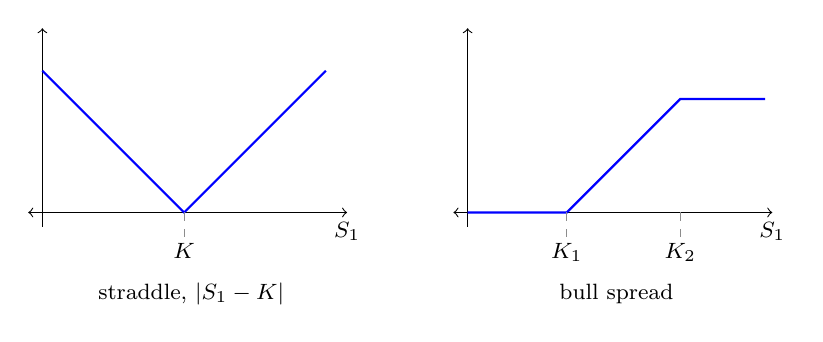
\begin{tikzpicture}[scale=0.9]
	\begin{scope}
		\draw[<->] (-0.2,0) -- (4.3,0) node[below] {\footnotesize $S_1$};
		\draw[->] (0,-0.2) -- (0,2.6);
		\draw[thick, color=blue] (0,2) -- (2,0) -- (4,2);
		\draw[dashed, color=black!45] (2,0) -- (2,-0.35);
		\node[below] at (2,-0.3) {\footnotesize $K$};
		\node at (2.1,-1.15) {\footnotesize straddle, $|S_1 - K|$};
	\end{scope}
	\begin{scope}[xshift=6cm]
		\draw[<->] (-0.2,0) -- (4.3,0) node[below] {\footnotesize $S_1$};
		\draw[->] (0,-0.2) -- (0,2.6);
		\draw[thick, color=blue] (0,0) -- (1.4,0) -- (3.0,1.6) -- (4.2,1.6);
		\draw[dashed, color=black!45] (1.4,0) -- (1.4,-0.35);
		\draw[dashed, color=black!45] (3.0,0) -- (3.0,-0.35);
		\node[below] at (1.4,-0.3) {\footnotesize $K_1$};
		\node[below] at (3.0,-0.3) {\footnotesize $K_2$};
		\node at (2.1,-1.15) {\footnotesize bull spread};
	\end{scope}
\end{tikzpicture}
\end{center}

A \vocab{straddle} is a call plus a put with the same strike, and pays off when the price moves a long way in either direction: it is a bet on volatility rather than on direction. A \vocab{bull spread} is a long call at strike $K_1$ and a short call at strike $K_2 > K_1$; it is a bet that the price will rise, but with the upside capped in exchange for a lower initial cost. Notice that the bull spread payoff is bounded, which is often what a regulator wants to see.

\subsection{No-Arbitrage Pricing}

Suppose the fundamental market (the $d$ assets and the bank) is arbitrage-free, and we add a claim with payout $Y$ and initial price $\pi$. When is the enlarged market still arbitrage-free?

\begin{theorem}[No-arbitrage pricing]\label{thm:na-pricing}
	Let the fundamental market be arbitrage-free. The augmented market containing the claim $(Y, \pi)$ is arbitrage-free if and only if
	$$
	\pi = \frac{1}{1+r}\EE_\QQ[Y]
	$$
	for some risk-neutral measure $\QQ$ of the fundamental market.
\end{theorem}

\begin{proof}
	Apply Theorem~\ref{thm:ftap1} to the augmented market, whose price vectors are $(S_0, \pi)^\top$ and $(S_1, Y)^\top$. The augmented market is arbitrage-free if and only if there is $\QQ \sim \PP$ with
	$$
	\frac{1}{1+r}\EE_\QQ\big[(S_1, Y)^\top\big] = (S_0, \pi)^\top.
	$$
	The first $d$ coordinates say exactly that $\QQ$ is risk-neutral for the fundamental market, and the last says $\pi = \EE_\QQ[Y]/(1+r)$.
\end{proof}

\begin{proposition}
	The set of no-arbitrage prices of a claim $Y$ is an interval.
\end{proposition}

\begin{proof}
	If $\QQ_0, \QQ_1$ are risk-neutral, so is $\QQ_t = t\QQ_1 + (1-t)\QQ_0$ for $t \in [0,1]$: it is a probability measure, it is equivalent to $\PP$ (its null sets are the common null sets), and $\EE_{\QQ_t}[S_1] = t\EE_{\QQ_1}[S_1] + (1-t)\EE_{\QQ_0}[S_1] = (1+r)S_0$. The corresponding price is $\pi_t = t\pi_1 + (1-t)\pi_0$, so the set of prices is convex.
\end{proof}

So a claim either has a unique no-arbitrage price, or a whole interval of them, in which case the model simply does not determine the price. The good case has a name.

\begin{definition}[Attainable claim]
	A claim $Y$ is \vocab{attainable} (or \vocab{replicable}) if $Y = a + b^\top S_1$ for some $a \in \R$, $b \in \R^d$; equivalently, if $Y \in \mathcal{X}(y)$ for some $y$. The portfolio achieving this is called a \vocab{replicating portfolio} or a \vocab{hedge}.
\end{definition}

\begin{theorem}\label{thm:attainable-price}
	If $Y \in \mathcal{X}(y)$ is attainable, then its unique no-arbitrage price is $y$, the initial cost of the replicating portfolio.
\end{theorem}

\begin{proof}
	Write $Y = a + b^\top S_1$, so $y = a/(1+r) + b^\top S_0$. For any risk-neutral $\QQ$,
	$$
	\frac{1}{1+r}\EE_\QQ[Y] = \frac{a}{1+r} + \frac{1}{1+r}b^\top \EE_\QQ[S_1] = \frac{a}{1+r} + b^\top S_0 = y,
	$$
	independently of $\QQ$. By Theorem~\ref{thm:na-pricing} this is the unique no-arbitrage price.
\end{proof}

This is the \vocab{law of one price}: two portfolios with the same payout must have the same price. Our very first example was an instance -- there the call was attainable, $Y = \tfrac13(S_1 - 4)$, and the price $\tfrac13$ was the cost of the hedge.

The converse of Theorem~\ref{thm:attainable-price} is also true, though we shall not prove it here (it is on the example sheet): a claim with a unique no-arbitrage price is attainable.

\subsection{Complete Markets}

\begin{definition}[Complete market]
	A market model is \vocab{complete} if every contingent claim is attainable.
\end{definition}

\begin{proposition}
	In a complete market model, $S_1$ takes at most $d+1$ values.
\end{proposition}

\begin{proof}
	Let $A_1,\dots,A_n$ be disjoint events of positive probability. The indicators $\ii_{A_1},\dots,\ii_{A_n}$ are linearly independent random variables. By completeness each $\ii_{A_i} = a_i + b_i^\top S_1$, so
	$$
	\vecspan\{\ii_{A_1},\dots,\ii_{A_n}\} \subseteq \vecspan\{1, S_1^1,\dots,S_1^d\},
	$$
	a space of dimension at most $d+1$. Hence $n \leq d+1$. As $S_1$ taking $n$ distinct values would give $n$ such disjoint events, the result follows.
\end{proof}

So completeness is a strong requirement: with one stock ($d=1$) it forces a binomial model. This is precisely why the binomial model is the workhorse of discrete-time finance.

\begin{theorem}[Second fundamental theorem of asset pricing]\label{thm:ftap2}
	An arbitrage-free market model is complete if and only if the risk-neutral measure is unique.
\end{theorem}

\begin{proof}
	($\Rightarrow$) Suppose the market is complete and $\QQ_0, \QQ_1$ are both risk-neutral. Set
	$$
	Y = \frac{\dd\QQ_1}{\dP} - \frac{\dd\QQ_0}{\dP},
	$$
	which is a bounded-below claim (in a complete market $S_1$ takes finitely many values, so $Y$ is a genuine random variable and everything is integrable). Since $Y$ is attainable, write $Y = a + b^\top S_1$; then for $i = 0,1$,
	$$
	\EE_{\QQ_i}[Y] = a + b^\top\EE_{\QQ_i}[S_1] = a + (1+r)b^\top S_0,
	$$
	the same value for both. But
	$$
	\EE_{\QQ_1}[Y] - \EE_{\QQ_0}[Y] = \EE_\PP\left[\left(\frac{\dd \QQ_1}{\dP} - \frac{\dd\QQ_0}{\dP}\right)Y\right] = \EE_\PP[Y^2],
	$$
	so $\EE_\PP[Y^2] = 0$ and hence $Y = 0$ a.s., i.e.\ $\QQ_0 = \QQ_1$.

	($\Leftarrow$) If the risk-neutral measure is unique then by Theorem~\ref{thm:na-pricing} every claim has exactly one no-arbitrage price, and hence (by the converse to Theorem~\ref{thm:attainable-price}) is attainable.
\end{proof}

\begin{example}
	Return to Example~\ref{ex:one-period-binom}. If $a < r < b$ the model is arbitrage-free with a unique risk-neutral measure $q = (r-a)/(b-a)$, hence complete: every claim $Y = g(S_1)$ is replicable, and
	$$
	\pi = \frac{1}{1+r}\Big(q\,g((1+b)S_0) + (1-q)\,g((1+a)S_0)\Big).
	$$
	The replicating portfolio is obtained by solving two linear equations in two unknowns; the number of shares held is
	$$
	\theta = \frac{g((1+b)S_0) - g((1+a)S_0)}{(b-a)S_0},
	$$
	the ratio of the change in payout to the change in stock price. This quantity will reappear as the \emph{delta} of the claim, and it is the single most important number in practical derivative trading.
\end{example}

\subsection{Utility Indifference Pricing}

Theorem~\ref{thm:na-pricing} pins down the price of a claim only when the claim is attainable. When it is not, we must go back to preferences. This subsection is a little more technical and may be skipped on a first reading, but it explains \emph{why} the risk-neutral price is the right answer even in incomplete markets, at least for small trades.

\begin{definition}[Indifference price]
	Fix a utility $U$ and initial wealth $x$. The \vocab{utility indifference price} (or \vocab{reservation bid price}) of a claim $Y$ is the largest $\pi$ with
	$$
	\sup\{\EE[U(X+Y)] : X \in \mathcal{X}(x - \pi)\} \geq \sup\{\EE[U(X)] : X \in \mathcal{X}(x)\}.
	$$
\end{definition}

In words -- the most the agent would pay for $Y$ while remaining at least as happy as if they had not bought it. We write $F_Y(\pi)$ for the left-hand side; note that $X \in \mathcal{X}(x-\pi)$ if and only if $X + (1+r)\pi \in \mathcal{X}(x)$, so
$$
F_Y(\pi) = \sup\{\EE[U(X - (1+r)\pi + Y)] : X \in \mathcal{X}(x)\},
$$
which is decreasing and (given mild regularity) continuous in $\pi$, with $F_Y(\mp\infty) = U(\pm\infty)$. Thus $\pi(Y)$ is the unique solution of $F_Y(\pi) = F_0(0)$.

\begin{theorem}
	The map $Y \mapsto \pi(Y)$ is concave.
\end{theorem}

\begin{proof}
	Fix claims $Y_0, Y_1$ and $t \in [0,1]$, and set $Y_t = tY_1 + (1-t)Y_0$. Let $X_i$ attain the supremum defining $F_{Y_i}(\pi(Y_i))$ for $i = 0,1$. Then $tX_1 + (1-t)X_0 \in \mathcal{X}(x - t\pi(Y_1) - (1-t)\pi(Y_0))$ by linearity, and so, using concavity of $U$,
	\begin{align*}
		F_{Y_t}(\pi(Y_t)) &= F_0(0) = tF_{Y_1}(\pi(Y_1)) + (1-t)F_{Y_0}(\pi(Y_0))\\
		&= t\,\EE[U(X_1 + Y_1)] + (1-t)\,\EE[U(X_0+Y_0)]\\
		&\leq \EE\big[U(tX_1 + (1-t)X_0 + Y_t)\big]\\
		&\leq F_{Y_t}\big(t\pi(Y_1) + (1-t)\pi(Y_0)\big).
	\end{align*}
	Since $F_{Y_t}$ is decreasing, $\pi(Y_t) \geq t\pi(Y_1) + (1-t)\pi(Y_0)$.
\end{proof}

Concavity says that an investor values diversification: half of one claim plus half of another is worth at least the average of the two. It also implies that $t \mapsto \pi(tY)/t$ is decreasing, so the limit
$$
\pi_0 := \lim_{t\downarrow 0}\frac{\pi(tY)}{t}
$$
exists. This is the \vocab{marginal} price of the claim -- the price per unit for an infinitesimally small trade.

\begin{lemma}[Supporting hyperplane]\label{lem:supporting}
	If $U$ is concave and differentiable then $U(y) - U(x) \leq U'(x)(y-x)$ for all $x,y$.
\end{lemma}

\begin{proof}
	For $x < x + \epsilon < y$, concavity of $U$ gives that the chord slopes decrease, so
	$$
	\frac{U(y)-U(x)}{y-x} \leq \frac{U(x+\epsilon)-U(x)}{\epsilon}.
	$$
	Letting $\epsilon \downarrow 0$ gives the claim, and the case $y < x$ is symmetric.
\end{proof}

\begin{lemma}\label{lem:foc-with-claim}
	If $X^*$ maximises $\EE[U(X+Y)]$ over $X \in \mathcal{X}(x)$, then $\EE[U'(X^*+Y)\,\xi] = 0$; consequently $\EE[U'(X^*+Y)(X^* - X)] = 0$ for all $X \in \mathcal{X}(x)$.
\end{lemma}

\begin{proof}
	Identical to Theorem~\ref{thm:foc}, differentiating in $\theta$. The second claim follows since $X^* - X$ is of the form $\eta^\top\xi$.
\end{proof}

\begin{theorem}[Marginal pricing]\label{thm:marginal}
	Let $X_0$ maximise $\EE[U(X)]$ over $X \in \mathcal{X}(x)$. Then
	$$
	\pi_0 = \frac{\EE[U'(X_0)Y]}{(1+r)\,\EE[U'(X_0)]} = \EE[ZY],
	$$
	where $Z$ is the state price density of Theorem~\ref{thm:spd-from-utility}.
\end{theorem}

\begin{proof}
	Write $\pi_t = \pi(tY)/t$ and let $X_t$ maximise $\EE[U(X + tY)]$ over $X \in \mathcal{X}(x - t\pi_t)$. By definition of the indifference price, $\EE[U(X_t + tY)] = \EE[U(X_0)]$.

	For the upper bound, note that $X_0 - t\pi_t(1+r) \in \mathcal{X}(x - t\pi_t)$, so it is a candidate in the supremum defining $X_t$, whence
	$$
	0 = \frac{\EE[U(X_t+tY) - U(X_0)]}{t} \geq \frac{\EE[U(X_0 - t\pi_t(1+r)+tY) - U(X_0)]}{t} \xrightarrow[t\downarrow 0]{} \EE\big[U'(X_0)(Y - (1+r)\pi_0)\big]
	$$
	using $\pi_t \downarrow \pi_0$ and dominated convergence. So $\EE[U'(X_0)(Y - (1+r)\pi_0)] \leq 0$.

	For the lower bound, apply Lemma~\ref{lem:supporting} and then Lemma~\ref{lem:foc-with-claim}:
	\begin{align*}
		0 = \frac{\EE[U(X_t+tY)-U(X_0)]}{t} &\leq \frac{\EE[U'(X_0)(X_t + tY - X_0)]}{t}\\
		&= \EE\big[U'(X_0)(Y - (1+r)\pi_t)\big] + \frac{1}{t}\EE\big[U'(X_0)(X_t + t\pi_t(1+r) - X_0)\big]\\
		&= \EE\big[U'(X_0)(Y - (1+r)\pi_t)\big],
	\end{align*}
	since $X_t + t\pi_t(1+r) \in \mathcal{X}(x)$ and Lemma~\ref{lem:foc-with-claim} (with $Y=0$) makes the last expectation vanish. Letting $t \downarrow 0$ gives $\EE[U'(X_0)(Y-(1+r)\pi_0)] \geq 0$.

	Combining the two bounds gives equality, which rearranges to the stated formula.
\end{proof}

So for small trades the indifference price is linear, and the linear functional is given by a state price density -- equivalently, by a risk-neutral expectation. This is the sense in which risk-neutral pricing is the right answer even when replication is impossible: it is the first-order approximation to what an optimising agent would pay.

\section{Martingales in Discrete Time}

To do finance in more than one period we must be able to say what an agent knows at each time. The mathematical device for this is the $\sigma$-algebra, and the resulting theory -- conditional expectation and martingales -- is the technical backbone of everything that follows.

\subsection{Information and \texorpdfstring{$\sigma$}{sigma}-Algebras}

Suppose we toss a coin twice, so $\Omega = \{HH, HT, TH, TT\}$. After the first toss we know whether the outcome lies in $\{HH,HT\}$ or in $\{TH,TT\}$, but nothing more. So the events we can resolve are
$$
\mathcal{G} = \big\{\emptyset,\ \{HH,HT\},\ \{TH,TT\},\ \Omega\big\}.
$$
The general shape of such a collection is clear: if we can resolve $A$ we can resolve $A^c$; if we can resolve each of $A_1, A_2, \dots$ we can resolve $\bigcup_n A_n$; and we can always resolve $\emptyset$. That is exactly the definition of a $\sigma$-algebra.

\begin{definition}[$\sigma$-algebra]
	A \vocab{$\sigma$-algebra} on a set $\Omega$ is a collection $\mathcal{G}$ of subsets of $\Omega$ with $\emptyset \in \mathcal{G}$, closed under complements and under countable unions. A random variable $X$ is \vocab{$\mathcal{G}$-measurable} if $X^{-1}(B) \in \mathcal{G}$ for every Borel set $B \subseteq \R$; equivalently, if $\{X \leq x\} \in \mathcal{G}$ for every $x \in \R$.
\end{definition}

The intuition is: $\mathcal{G}$ is `the information available', and $X$ is $\mathcal{G}$-measurable if $X$ is known once that information is revealed. The two extreme cases are the \vocab{trivial $\sigma$-algebra} $\{\emptyset,\Omega\}$ (no information -- the only measurable random variables are constants) and the power set $2^\Omega$ (everything is known).

\begin{definition}
	The $\sigma$-algebra \vocab{generated} by a random variable $X$ is $\sigma(X) = \{X^{-1}(B) : B \text{ Borel}\}$, the smallest $\sigma$-algebra making $X$ measurable. More generally $\sigma(X_1,\dots,X_n)$ is the smallest $\sigma$-algebra making all of $X_1,\dots,X_n$ measurable.
\end{definition}

\begin{fact}
	A random variable $Y$ is $\sigma(X)$-measurable if and only if $Y = g(X)$ for some Borel measurable $g$.
\end{fact}

This is the precise sense in which `knowing $X$' means `knowing every function of $X$, and nothing else'. We shall use it without further comment.

\subsection{Conditional Expectation}

In Part IA Probability you defined $\EE[X \mid A] = \EE[X\ii_A]/\PP(A)$ for an event $A$ of positive probability, and $\EE[X \mid Y]$ for a discrete random variable $Y$ as the random variable taking value $\EE[X \mid Y = y]$ on $\{Y = y\}$. We now want to condition on a whole $\sigma$-algebra, including ones generated by continuous random variables where every individual event has probability zero. The trick is to characterise the answer rather than construct it.

Note first the key property of the discrete construction: if $f(y) = \EE[X \mid Y=y]$ then for every bounded $\sigma(Y)$-measurable $Z$,
$$
\EE[XZ] = \EE[f(Y)Z],
$$
as one checks by decomposing over the values of $Y$. We turn this into a definition.

\begin{definition}[Conditional expectation]
	Let $X$ be an integrable random variable on $(\Omega,\FF,\PP)$ and $\mathcal{G}\subseteq \FF$ a $\sigma$-algebra. A random variable $\tilde X$ is a \vocab{conditional expectation} of $X$ given $\mathcal{G}$ if
	\begin{enumerate}[label=(\roman*)]
		\item $\tilde X$ is $\mathcal{G}$-measurable and integrable;
		\item $\EE[XZ] = \EE[\tilde X Z]$ for every bounded $\mathcal{G}$-measurable $Z$.
	\end{enumerate}
\end{definition}

\begin{proposition}
	A conditional expectation exists and is almost surely unique. We write it $\EE[X \mid \mathcal{G}]$, and $\EE[X\mid Y] := \EE[X \mid \sigma(Y)]$.
\end{proposition}

\begin{proof}
	We prove uniqueness, existence being a genuinely measure-theoretic matter (it follows from the Radon--Nikodym theorem, or from the $L^2$ projection argument below). Suppose $\tilde X_0$ and $\tilde X_1$ both work. Take $Z = \ii_{\{\tilde X_0 < \tilde X_1\}}$, which is bounded and $\mathcal{G}$-measurable. Then
	$$
	\EE\big[(\tilde X_1 - \tilde X_0)\ii_{\{\tilde X_0 < \tilde X_1\}}\big] = \EE[XZ] - \EE[XZ] = 0.
	$$
	The integrand is non-negative and strictly positive on $\{\tilde X_0 < \tilde X_1\}$, so $\PP(\tilde X_0 < \tilde X_1) = 0$. By symmetry $\PP(\tilde X_0 > \tilde X_1) = 0$.
\end{proof}

The following interpretation is worth recording, since it explains why conditional expectation is `the best guess'.

\begin{proposition}[$L^2$ projection]
	Let $X$ be square integrable and $\tilde X = \EE[X\mid\mathcal{G}]$. Then for every square-integrable $\mathcal{G}$-measurable $Z$,
	$$
	\EE\big[(X-\tilde X)^2\big] \leq \EE\big[(X - Z)^2\big].
	$$
\end{proposition}

\begin{proof}
	Expand:
	$$
	\EE[(X-Z)^2] = \EE[(X - \tilde X)^2] + 2\EE\big[(X-\tilde X)(\tilde X - Z)\big] + \EE[(\tilde X - Z)^2].
	$$
	The middle term vanishes: $\tilde X - Z$ is $\mathcal{G}$-measurable, so the defining property gives $\EE[X(\tilde X - Z)] = \EE[\tilde X(\tilde X - Z)]$ (first for bounded $\tilde X - Z$, then in general by truncation). The last term is non-negative.
\end{proof}

So $\EE[X\mid\mathcal{G}]$ is the orthogonal projection of $X$ onto the closed subspace of $\mathcal{G}$-measurable square-integrable random variables. All the familiar properties now follow.

\begin{proposition}[Properties of conditional expectation]\label{prop:ce-props}
	Assume all the conditional expectations below are well defined. Then, almost surely:
	\begin{enumerate}[label=(\roman*)]
		\item (\emph{Linearity}) $\EE[aX + bY \mid \mathcal{G}] = a\EE[X\mid\mathcal{G}] + b\EE[Y\mid\mathcal{G}]$;
		\item (\emph{Taking out what is known}) if $Y$ is $\mathcal{G}$-measurable then $\EE[XY\mid\mathcal{G}] = Y\,\EE[X\mid\mathcal{G}]$;
		\item (\emph{Positivity}) if $X \geq 0$ a.s.\ then $\EE[X\mid\mathcal{G}]\geq 0$ a.s.;
		\item (\emph{Independence}) if $\sigma(X)$ is independent of $\mathcal{G}$ then $\EE[X\mid\mathcal{G}] = \EE[X]$;
		\item (\emph{Jensen}) if $f$ is convex then $\EE[f(X)\mid\mathcal{G}] \geq f(\EE[X\mid\mathcal{G}])$;
		\item (\emph{Tower property}) if $\mathcal{G}\subseteq\mathcal{H}\subseteq\FF$ then $\EE[\EE[X\mid\mathcal{H}]\mid\mathcal{G}] = \EE[X\mid\mathcal{G}]$.
	\end{enumerate}
\end{proposition}

\begin{proof}
	(i) Both sides are $\mathcal{G}$-measurable and satisfy the defining identity, so uniqueness applies. (ii) For bounded $\mathcal{G}$-measurable $Z$ we have $\EE[(XY)Z] = \EE[X(YZ)] = \EE[\EE[X\mid\mathcal{G}]YZ]$, since $YZ$ is $\mathcal{G}$-measurable (first for bounded $Y$, then by truncation).
	(iii) Take $Z = \ii_{\{\EE[X\mid\mathcal{G}]<0\}}$; then $\EE[\EE[X\mid\mathcal{G}]Z] = \EE[XZ]\geq 0$, whereas the left-hand side is $\leq 0$ and is $<0$ unless $\PP(\EE[X\mid\mathcal{G}]<0) = 0$.
	(iv) Immediate from the definition, since $\EE[XZ] = \EE[X]\EE[Z]$ for $\mathcal{G}$-measurable $Z$.
	(v) A convex $f$ satisfies $f(y)\geq f(x) + \lambda(x)(y-x)$ for a suitable $\lambda(x)$; put $x = \EE[X\mid\mathcal{G}]$, $y = X$ and condition.
	(vi) $\EE[X\mid\mathcal{G}]$ is $\mathcal{H}$-measurable so equals its own conditional expectation given $\mathcal{H}$; for the other order, any bounded $\mathcal{G}$-measurable $Z$ is $\mathcal{H}$-measurable, so $\EE[\EE[X\mid\mathcal{H}]Z] = \EE[XZ]$.
\end{proof}

\begin{example}
	Let $(A_n)_{n\geq1}$ partition $\Omega$ with $\PP(A_n) > 0$ and let $\mathcal{G} = \sigma(A_1,A_2,\dots)$. A random variable is $\mathcal{G}$-measurable exactly when it is constant on each $A_n$, and
	$$
	\EE[X\mid\mathcal{G}] = \sum_n \EE[X\mid A_n]\,\ii_{A_n},
	$$
	which recovers the Part IA definition.
\end{example}

\subsection{Filtrations and Martingales}

\begin{definition}[Filtration]
	A \vocab{filtration} on $(\Omega,\FF)$ is an increasing sequence $(\FF_n)_{n\geq 0}$ of $\sigma$-algebras, $\FF_0 \subseteq \FF_1 \subseteq \cdots \subseteq \FF$. A stochastic process $(X_n)_{n\geq0}$ is \vocab{adapted} to $(\FF_n)$ if $X_n$ is $\FF_n$-measurable for every $n$. The filtration \vocab{generated} by a process $(X_n)$ is $\FF_n = \sigma(X_0,\dots,X_n)$.
\end{definition}

We adopt the convention that $\FF_0 = \{\emptyset,\Omega\}$ is trivial, so $X_0$ is a constant and $\EE[Z\mid\FF_0] = \EE[Z]$ for every integrable $Z$.

\begin{definition}[Martingale]
	An adapted, integrable process $(X_n)_{n\geq0}$ is a \vocab{martingale} with respect to $(\FF_n)$ if
	$$
	\EE[X_n \mid \FF_{n-1}] = X_{n-1} \qquad \text{for all } n \geq 1.
	$$
	It is a \vocab{supermartingale} if $\EE[X_n\mid\FF_{n-1}] \leq X_{n-1}$ and a \vocab{submartingale} if $\EE[X_n\mid\FF_{n-1}]\geq X_{n-1}$.
\end{definition}

A martingale is a fair game: given everything you know today, your expected fortune tomorrow is exactly your fortune today. A supermartingale is a game which is unfavourable to you (it goes \emph{down} on average -- the terminology is unfortunate but universal), and a submartingale is a favourable one.

\begin{proposition}\label{prop:mart-equiv}
	For an adapted integrable process $(X_n)$ the following are equivalent:
	\begin{enumerate}[label=(\roman*)]
		\item $(X_n)$ is a martingale;
		\item $\EE[X_n - X_{n-1}\mid\FF_{n-1}] = 0$ for all $n \geq 1$;
		\item $\EE[X_n\mid\FF_m] = X_m$ for all $0 \leq m \leq n$.
	\end{enumerate}
\end{proposition}

\begin{proof}
	(i) $\iff$ (ii) is immediate from linearity, and (iii) $\implies$ (i) is the case $m = n-1$. For (i) $\implies$ (iii), induct on $n - m$ using the tower property:
	$$
	\EE[X_{n}\mid\FF_m] = \EE\big[\EE[X_{n}\mid\FF_{n-1}]\,\big|\,\FF_m\big] = \EE[X_{n-1}\mid\FF_m] = X_m. \qedhere
	$$
\end{proof}

Condition (iii) makes no reference to `the previous time step', and so is the definition that generalises to continuous time.

\begin{example}[Martingales built backwards]
	Let $Z$ be integrable and $(\FF_n)$ a filtration. Then $X_n = \EE[Z\mid\FF_n]$ is a martingale. Integrability follows from conditional Jensen, $\EE|X_n| \leq \EE[\EE[|Z|\mid\FF_n]] = \EE|Z| < \infty$, and the martingale property is the tower property. Every martingale on a finite horizon arises this way, with $Z = X_N$.
\end{example}

\begin{example}[Martingales built forwards]
	\begin{enumerate}[label=(\roman*)]
		\item Let $(Y_n)$ be independent integrable random variables with $\EE[Y_n] = 0$, and let $\FF_n = \sigma(Y_1,\dots,Y_n)$. Then $S_0 = 0$, $S_n = Y_1 + \dots + Y_n$ defines a martingale, since
		$$
		\EE[S_n - S_{n-1}\mid\FF_{n-1}] = \EE[Y_n\mid\FF_{n-1}] = \EE[Y_n] = 0
		$$
		by independence. In particular the simple symmetric random walk is a martingale.
		\item If instead $(Y_n)$ are independent, positive, with $\EE[Y_n]=1$, then $M_0 = 1$, $M_n = Y_1\cdots Y_n$ is a martingale by the same computation.
		\item If $(S_n)$ is a simple symmetric random walk then $Q_n = S_n^2 - n$ is a martingale: indeed $\EE[S_n^2\mid\FF_{n-1}] = S_{n-1}^2 + 2S_{n-1}\EE[Y_n] + \EE[Y_n^2] = S_{n-1}^2 + 1$.
	\end{enumerate}
\end{example}

The definition immediately relevant to us is the following, which we shall justify in \S6.

\begin{definition}[Risk-neutral measure, multi-period]
	For a multi-period market with prices $(S_n)_{n\geq0}$ adapted to $(\FF_n)$ and interest rate $r$, a probability measure $\QQ\sim\PP$ is \vocab{risk-neutral} if the discounted price process $\big(S_n/(1+r)^n\big)_{n \geq 0}$ is a $\QQ$-martingale, i.e.\ if
	$$
	\EE_\QQ[S_n \mid \FF_{n-1}] = (1+r)S_{n-1}\qquad \text{for all } n\geq1.
	$$
\end{definition}

\subsection{Stopping Times and Optional Stopping}

\begin{definition}[Stopping time]
	A random variable $T$ taking values in $\{0,1,2,\dots\}\cup\{\infty\}$ is a \vocab{stopping time} for the filtration $(\FF_n)$ if $\{T \leq n\}\in\FF_n$ for every $n$.
\end{definition}

The condition says that we can decide whether to stop at time $n$ using only information available at time $n$ -- no peeking into the future.

\begin{example}
	\begin{enumerate}[label=(\roman*)]
		\item If $(X_n)$ is adapted then the first hitting time $T = \inf\{n\geq 0 : X_n > 0\}$ (with $\inf\emptyset = \infty$) is a stopping time, since $\{T \leq n\} = \bigcup_{k\leq n}\{X_k > 0\}\in\FF_n$.
		\item The last time $T = \sup\{n \geq 0 : X_n > 0\}$ is generally \emph{not} a stopping time: $\{T\leq n\} = \bigcap_{k>n}\{X_k \leq 0\}$ requires knowledge of the whole future. `Sell at the top' is not an implementable strategy.
	\end{enumerate}
\end{example}

\begin{definition}[Stopped process]
	Given a process $X$ and a random time $T$, the \vocab{stopped process} $X^T$ is defined by
	$$
	X_n^T = X_{n\wedge T} = X_0 + \sum_{k=1}^n \ii_{\{k\leq T\}}(X_k - X_{k-1}).
	$$
\end{definition}

\begin{proposition}
	If $X$ is integrable and adapted and $T$ is a stopping time, then $X^T$ is integrable and adapted.
\end{proposition}

\begin{proof}
	Integrability follows from the triangle inequality applied to the sum. For adaptedness, note $\{k \leq T\} = \{T \leq k-1\}^c \in\FF_{k-1}\subseteq\FF_n$ for $k \leq n$, and $X_k - X_{k-1}$ is $\FF_n$-measurable.
\end{proof}

\begin{theorem}[Optional sampling]\label{thm:optional-sampling}
	Let $X$ be a martingale and $T$ a stopping time. Then $X^T$ is a martingale. In particular, if $T \leq N$ almost surely for some constant $N$, then $\EE[X_T] = X_0$.
\end{theorem}

\begin{proof}
	We know $X^T$ is adapted and integrable, so it remains to compute, for $n\geq1$,
	$$
	\EE\big[X_n^T - X_{n-1}^T \mid\FF_{n-1}\big] = \EE\big[\ii_{\{n\leq T\}}(X_n - X_{n-1})\mid\FF_{n-1}\big] = \ii_{\{n\leq T\}}\,\EE[X_n - X_{n-1}\mid\FF_{n-1}] = 0,
	$$
	where we took out the $\FF_{n-1}$-measurable factor $\ii_{\{n\leq T\}}$. If $T \leq N$ a.s.\ then $X_T = X_{T\wedge N} = X_N^T$, and $\EE[X^T_N] = X^T_0 = X_0$.
\end{proof}

The boundedness hypothesis is essential.

\begin{example}[Why boundedness matters]\label{ex:doubling}
	Let $(S_n)$ be a simple symmetric random walk from $0$ and let $T = \inf\{n\geq0 : S_n = b\}$ for $b > 0$. From Part IB Markov Chains we know the walk is recurrent, so $T < \infty$ a.s.\ and $S_T = b$. Then $\EE[S_T] = b \neq 0 = S_0$. Optional sampling fails, because $T$ is unbounded and unboundedly large excursions occur before $T$.

	This is not a mere technicality: it is the martingale-theoretic reason why the `double your bet until you win' strategy does not actually work. It requires an unbounded amount of credit, and $\EE[\min_{n \leq T}S_n] = -\infty$.
\end{example}

To handle unbounded stopping times we need an integrability condition.

\begin{theorem}[Optional stopping]\label{thm:optional-stopping}
	Let $X$ be a martingale and $T$ a stopping time with $T<\infty$ a.s. Suppose there is an integrable random variable $Y$ with $|X^T_n| \leq Y$ for all $n$. Then $X_n^T \to X_T$ a.s.\ and $\EE[X_T] = X_0$.
\end{theorem}

\begin{proof}
	Since $T<\infty$ a.s., $X_n^T = X_T$ for all $n \geq T$, giving almost sure convergence. By Theorem~\ref{thm:optional-sampling}, $\EE[X_n^T] = X_0$ for every $n$; the dominated convergence theorem lets us pass to the limit.
\end{proof}

In particular the conclusion holds if $T$ is bounded, or if $T$ is integrable and the increments of $X$ are bounded, or if $X^T$ is bounded. Let us see the last of these in action.

\begin{example}[Gambler's ruin, again]
	Let $(S_n)$ be a simple symmetric random walk from $0$ and $T = \inf\{n \geq 0: S_n \in \{-a,b\}\}$ for integers $a,b>0$. Then $|S_n^T|\leq \max(a,b)$, and $T<\infty$ a.s.\ (again by recurrence), so Theorem~\ref{thm:optional-stopping} gives
	$$
	0 = \EE[S_T] = -a\,\PP(S_T = -a) + b\,\PP(S_T = b).
	$$
	With $\PP(S_T=-a)+\PP(S_T=b)=1$ this yields
	$$
	\PP(S_T = -a) = \frac{b}{a+b},\qquad \PP(S_T = b) = \frac{a}{a+b},
	$$
	which is the gambler's ruin formula from Part IA. Applying the same argument to the martingale $Q_n = S_n^2 - n$ and the bounded stopping time $T\wedge n$,
	$$
	\EE[S^2_{T\wedge n}] = \EE[T \wedge n].
	$$
	The right-hand side increases to $\EE[T]$ by monotone convergence and the left-hand side converges to $\EE[S_T^2]$ by dominated convergence, so
	$$
	\EE[T] = \EE[S_T^2] = a^2\frac{a}{a+b}\cdot\frac{b}{a} + b^2 \frac{a}{a+b} = ab,
	$$
	after simplification: the expected duration is $ab$.
\end{example}

\subsection{Martingale Transforms}

\begin{definition}[Previsible process]
	A process $(H_n)_{n\geq1}$ is \vocab{previsible} (or \vocab{predictable}) for $(\FF_n)$ if $H_n$ is $\FF_{n-1}$-measurable for every $n \geq 1$.
\end{definition}

\begin{definition}[Martingale transform]
	The \vocab{martingale transform} of $X$ by $H$ is the process
	$$
	(H\cdot X)_n = \sum_{k=1}^n H_k(X_k - X_{k-1}), \qquad (H\cdot X)_0 = 0.
	$$
\end{definition}

Think of $X_k - X_{k-1}$ as the winnings per unit stake in game $k$ and $H_k$ as the stake, chosen before the game is played. Then $(H\cdot X)_n$ is the total winnings. The martingale transform is the discrete-time ancestor of the stochastic integral $\int H \dd X$.

\begin{theorem}[You cannot beat the system]\label{thm:transform}
	Let $H$ be previsible and bounded.
	\begin{enumerate}[label=(\roman*)]
		\item If $X$ is a martingale then so is $H \cdot X$.
		\item If $X$ is a supermartingale and $H \geq 0$, then $H\cdot X$ is a supermartingale.
	\end{enumerate}
\end{theorem}

\begin{proof}
	In both cases $H\cdot X$ is adapted (since $H_k$ is $\FF_{k-1}$-measurable and $X$ adapted) and integrable (since $H$ is bounded). Then
	$$
	\EE\big[(H\cdot X)_n - (H\cdot X)_{n-1}\mid\FF_{n-1}\big] = \EE\big[H_n(X_n-X_{n-1})\mid\FF_{n-1}\big] = H_n\,\EE[X_n - X_{n-1}\mid\FF_{n-1}],
	$$
	which is $0$ in case (i) and $\leq 0$ in case (ii) as $H_n \geq 0$.
\end{proof}

The name is apt: no gambling strategy, however clever, can turn a fair game into a favourable one, provided your stakes are chosen without knowledge of the future and you are not allowed to bet unboundedly.

Notice that the stopped process is a special case: $X^T - X_0 = H\cdot X$ with $H_k = \ii_{\{k\leq T\}}$, which is previsible precisely because $T$ is a stopping time.

\subsection{Supermartingales and the Snell Envelope}

For optimal stopping problems we need the supermartingale analogue of optional sampling.

\begin{theorem}[Optional sampling for supermartingales]\label{thm:oss-super}
	Let $X$ be a supermartingale and let $S \leq T$ be bounded stopping times. Then $\EE[X_S]\geq\EE[X_T]$.
\end{theorem}

\begin{proof}
	Suppose $T \leq N$. Writing the difference as a sum,
	$$
	X_{N\wedge T} - X_{N \wedge S} = \sum_{k=1}^{N}\ii_{\{S < k \leq T\}}(X_k - X_{k-1}).
	$$
	Now $\{S<k\} = \{S\leq k-1\}\in\FF_{k-1}$ and $\{k\leq T\} = \{T\leq k-1\}^c\in\FF_{k-1}$, so $\ii_{\{S<k\leq T\}}$ is $\FF_{k-1}$-measurable. Hence
	$$
	\EE[X_T - X_S] = \sum_{k=1}^N\EE\Big[\ii_{\{S<k\leq T\}}\,\EE[X_k - X_{k-1}\mid\FF_{k-1}]\Big] \leq 0,
	$$
	since each conditional expectation is $\leq 0$ and the indicator is non-negative.
\end{proof}

Now consider the following optimal stopping problem. Fix a horizon $N$, an adapted process $(Y_n)_{0\leq n \leq N}$ of payouts, and ask for
$$
\sup\big\{\EE[Y_T] : T \text{ a stopping time with } T \leq N\big\}.
$$

\begin{definition}[Snell envelope]
	The \vocab{Snell envelope} of $(Y_n)_{n \leq N}$ is the process defined by backward recursion
	$$
	Z_N = Y_N, \qquad Z_{n-1} = \max\big\{Y_{n-1},\ \EE[Z_n\mid\FF_{n-1}]\big\}.
	$$
\end{definition}

At each time we compare the payout from stopping now with the expected value of carrying on optimally; the Snell envelope is the value of the problem.

\begin{theorem}[Optimal stopping]\label{thm:snell}
	The Snell envelope $(Z_n)$ is the smallest supermartingale dominating $(Y_n)$. Moreover
	$$
	T^* = \min\{n \geq 0 : Z_n = Y_n\}
	$$
	is an optimal stopping time, and $Z_0 = \EE[Y_{T^*}] = \sup_{T\leq N}\EE[Y_T]$.
\end{theorem}

\begin{proof}
	By construction $Z_n \geq Y_n$ and $Z_{n-1}\geq\EE[Z_n\mid\FF_{n-1}]$, so $Z$ is a supermartingale dominating $Y$. If $W$ is any other such supermartingale then $W_N \geq Y_N = Z_N$, and inductively
	$$
	W_{n-1}\geq\max\{Y_{n-1}, \EE[W_n\mid\FF_{n-1}]\} \geq \max\{Y_{n-1},\EE[Z_n\mid\FF_{n-1}]\} = Z_{n-1},
	$$
	so $Z$ is the smallest.

	For any stopping time $T \leq N$, Theorem~\ref{thm:oss-super} applied with $S = 0$ gives $\EE[Y_T]\leq\EE[Z_T]\leq Z_0$.

	It remains to show equality for $T^*$. The definition of $T^*$ gives $Z_n > Y_n$ for $n < T^*$, so on $\{n \leq T^*\}$ we have $Z_{n-1} = \EE[Z_n\mid\FF_{n-1}]$ for $n\leq T^*$; hence the stopped process $Z^{T^*}$ satisfies
	$$
	\EE[Z^{T^*}_n - Z^{T^*}_{n-1}\mid\FF_{n-1}] = \ii_{\{n\leq T^*\}}\big(\EE[Z_n\mid\FF_{n-1}] - Z_{n-1}\big) = 0,
	$$
	so $Z^{T^*}$ is a martingale. Therefore $Z_0 = \EE[Z^{T^*}_N] = \EE[Z_{T^*}] = \EE[Y_{T^*}]$, using $Z_{T^*} = Y_{T^*}$.
\end{proof}

This is the engine that will price American options. Note the structure of the answer: one solves a backward recursion, and the optimal rule is `stop as soon as the payout from stopping equals the value of the problem'.

\subsection{Convergence}

We record, without proof, the two convergence results that we shall occasionally need. The first is the martingale convergence theorem; you will meet it properly in Part II Probability and Measure.

\begin{theorem}[Martingale convergence]
	Let $(X_n)$ be a martingale bounded in $L^1$, i.e.\ $\sup_n\EE|X_n| < \infty$. Then $X_n \to X_\infty$ almost surely for some integrable $X_\infty$.
\end{theorem}

In general $\EE[X_\infty] \neq X_0$: Example~\ref{ex:doubling} is a counterexample if one truncates suitably. What is needed for the limit to be `honest' is uniform integrability, and then $X_n = \EE[X_\infty\mid\FF_n]$ for all $n$.

\begin{theorem}[Monotone and dominated convergence]
	If $0\leq X_n \leq X_{n+1}$ a.s.\ then $\EE[X_n]\to\EE[\lim_n X_n]$. If $X_n \to X$ a.s.\ and $|X_n|\leq Y$ for an integrable $Y$, then $\EE[X_n]\to\EE[X]$.
\end{theorem}

\section{Multi-Period Models}

We now let the market run for $N$ periods. The state space carries a filtration $(\FF_n)_{0\leq n\leq N}$, prices $(S_n)$ are adapted, and the bank account grows by a factor $1+r$ each period. Everything from \S4 will survive, with `random variable' replaced by `adapted process' and `expectation' by `conditional expectation'.

\subsection{Self-Financing Portfolios}

Let $\theta_n \in \R^d$ be the portfolio of risky assets held over the interval $(n-1,n]$, and $\theta_n^0$ the amount in the bank over the same interval. These must be chosen at time $n-1$, so we require $(\theta_n)_{n\geq1}$ to be \emph{previsible}. Let $X_n$ be the agent's wealth at time $n$.

\begin{definition}[Self-financing]
	A previsible portfolio process $(\theta_n)$ is \vocab{self-financing} if no money is added to or removed from the portfolio after time $0$; that is, if
	$$
	X_{n-1} = \theta_n^0 + \theta_n^\top S_{n-1} \qquad \text{and}\qquad X_n = \theta_n^0(1+r) + \theta_n^\top S_n
	$$
	for all $n \geq 1$.
\end{definition}

Eliminating $\theta_n^0$ exactly as in the one-period case gives the wealth recursion
$$
X_n = (1+r)X_{n-1} + \theta_n^\top\big(S_n - (1+r)S_{n-1}\big).
$$
It is neater in discounted terms. Write $\tilde X_n = X_n/(1+r)^n$ and $\tilde S_n = S_n/(1+r)^n$ for the discounted wealth and prices, i.e.\ prices measured in units of the bank account rather than in pounds. Dividing the recursion by $(1+r)^n$,
$$
\tilde X_n - \tilde X_{n-1} = \theta_n^\top\big(\tilde S_n - \tilde S_{n-1}\big),
$$
and summing,
$$
\boxed{\;\tilde X_n = X_0 + \sum_{k=1}^n \theta_k^\top\big(\tilde S_k - \tilde S_{k-1}\big) = X_0 + (\theta\cdot\tilde S)_n.\;}
$$
In other words -- the discounted wealth of a self-financing strategy is the initial wealth plus the martingale transform of the strategy against the discounted prices. Theorem~\ref{thm:transform} now does an enormous amount of work for us.

\begin{remark}
	The change from pounds to units of the bank account is our first \vocab{change of numeraire}. A \vocab{numeraire} is any asset with strictly positive price which we use as the unit of account; discounting is the statement that in the numeraire of the bank account the riskless asset has constant price $1$. Choosing a different numeraire will be useful in \S9.
\end{remark}

\subsection{Arbitrage in Multi-Period Models}

\begin{definition}[Arbitrage]
	A previsible process $(\theta_n)_{1\leq n\leq N}$ is an \vocab{arbitrage} if the terminal discounted gain $G = \sum_{k=1}^N \theta_k^\top(\tilde S_k - \tilde S_{k-1})$ satisfies
	$$
	\PP(G \geq 0) = 1 \qquad\text{and}\qquad \PP(G>0)>0.
	$$
\end{definition}

\begin{theorem}[Fundamental theorem of asset pricing]\label{thm:ftap-multi}
	A finite-horizon market model admits no arbitrage if and only if there exists a risk-neutral measure, that is, a $\QQ\sim\PP$ under which $(\tilde S_n)_{0\leq n\leq N}$ is a martingale.
\end{theorem}

\begin{proof}
	($\Leftarrow$) Let $\QQ$ be risk-neutral and let $\theta$ be previsible and bounded. By Theorem~\ref{thm:transform} the discounted wealth $\tilde X_n = X_0 + (\theta\cdot\tilde S)_n$ is a $\QQ$-martingale, so
	$$
	\EE_\QQ[G] = \EE_\QQ[\tilde X_N] - X_0 = 0.
	$$
	If $\theta$ were an arbitrage then $G \geq 0$ $\PP$-a.s., hence $\QQ$-a.s.\ since $\PP\sim\QQ$; a non-negative random variable of zero mean vanishes a.s., so $G = 0$ $\QQ$-a.s.\ and therefore $\PP$-a.s., contradicting $\PP(G>0)>0$. (For unbounded $\theta$ one first localises using the stopping times $T_m = \inf\{n : \|\theta_{n+1}\|>m\}$ and then lets $m\to\infty$.)

	($\Rightarrow$) Conversely, suppose there is no arbitrage. Then in particular, for each $n$ there is no one-period arbitrage conditional on $\FF_{n-1}$: if $\eta$ were an $\FF_{n-1}$-measurable random vector with $\eta^\top(\tilde S_n - \tilde S_{n-1})\geq 0$ a.s.\ and positive with positive probability, then the strategy which is $\eta$ at time $n$ and zero otherwise would be an arbitrage. Applying the one-period Theorem~\ref{thm:ftap1} conditionally on $\FF_{n-1}$ produces, for each $n$, a strictly positive $\FF_n$-measurable $Y_n$ with $\EE[Y_n\mid\FF_{n-1}] = 1$ and $\EE[Y_n \tilde S_n \mid \FF_{n-1}] = \tilde S_{n-1}$. Setting $\dQ/\dP = \prod_{n=1}^N Y_n$ defines an equivalent measure, and a short computation with the tower property shows $\tilde S$ is a $\QQ$-martingale.
\end{proof}

\begin{theorem}[Second fundamental theorem]
	An arbitrage-free model is complete -- every $\FF_N$-measurable claim $Y$ is replicable by a self-financing strategy -- if and only if the risk-neutral measure is unique. In that case the unique time-$n$ no-arbitrage price of a claim $Y$ payable at time $N$ is
	$$
	\pi_n = \frac{1}{(1+r)^{N-n}}\,\EE_\QQ\big[Y \mid \FF_n\big].
	$$
\end{theorem}

\begin{proof}[Proof sketch]
	The equivalence is proved exactly as in Theorem~\ref{thm:ftap2}. For the formula, note that $(\pi_n/(1+r)^n)$ must be a $\QQ$-martingale (else the augmented market has an arbitrage, by the argument of Theorem~\ref{thm:na-pricing} applied at each time), with terminal value $Y/(1+r)^N$; and a martingale is determined by its terminal value via Proposition~\ref{prop:mart-equiv}(iii).
\end{proof}

\subsection{The Binomial Model}

We now specialise to the model in which every computation can be carried out explicitly.

\begin{definition}[Cox--Ross--Rubinstein model]
	Take $d = 1$ and let $(\xi_n)_{n \geq 1}$ be i.i.d.\ with
	$$
	\PP(\xi = 1+b) = p = 1 - \PP(\xi = 1+a), \qquad a < b,\ p \in (0,1),
	$$
	and set $S_n = S_{n-1}\xi_n = S_0\xi_1\cdots\xi_n$, with $(\FF_n)$ the filtration generated by $(S_n)$. This is the \vocab{binomial} or \vocab{Cox--Ross--Rubinstein} model.
\end{definition}

\begin{proposition}\label{prop:crr-na}
	The binomial model is arbitrage-free if and only if $a < r < b$, and in that case the risk-neutral measure is unique: under $\QQ$ the $\xi_n$ are i.i.d.\ with
	$$
	\QQ(\xi = 1+b) = q = \frac{r-a}{b-a}.
	$$
	Consequently the model is complete.
\end{proposition}

\begin{proof}
	If $r \leq a$ then $\theta_1 = 1$ (buy a share, hold it one period, do nothing thereafter) is an arbitrage, since $S_1 - (1+r)S_0 \geq (1+a-1-r)S_0\geq0$ with strict inequality when $\xi_1 = 1+b$. If $r \geq b$ then $\theta_1 = -1$ is an arbitrage. Conversely, suppose $a<r<b$. A measure $\QQ$ under which $\tilde S$ is a martingale must satisfy $\EE_\QQ[\xi_n \mid \FF_{n-1}] = 1+r$; since $\xi_n$ takes two values this determines the conditional law of $\xi_n$ given $\FF_{n-1}$ to be the two-point law with mass $q = (r-a)/(b-a)$ at $1+b$, and $q\in(0,1)$ exactly when $a<r<b$. This makes the $\xi_n$ i.i.d.\ under $\QQ$, and conversely that choice visibly works. Uniqueness plus the second fundamental theorem gives completeness.
\end{proof}

The price process is \vocab{recombining}: an up-move followed by a down-move gives the same price as a down followed by an up, so after $n$ steps there are only $n+1$ possible prices rather than $2^n$. Here is the tree we shall use as a running example, with
$$
S_0 = 100,\quad 1+b = 1.2,\quad 1+a = 0.9,\quad r = 0.05,\quad N = 3,
$$
so that $q = (0.05+0.1)/(0.2+0.1) = \tfrac12$.

\begin{center}
\begin{tikzpicture}[scale=1.0]
	\tikzset{pnode/.style={inner sep=1.5pt, fill=white, font=\footnotesize}}
	\foreach \n/\k in {0/0,1/0,1/1,2/0,2/1,2/2}{
	}
	% edges
	\draw[thin] (0,0) -- (2.7,0.95); \draw[thin] (0,0) -- (2.7,-0.95);
	\draw[thin] (2.7,0.95) -- (5.4,1.9); \draw[thin] (2.7,0.95) -- (5.4,0);
	\draw[thin] (2.7,-0.95) -- (5.4,0); \draw[thin] (2.7,-0.95) -- (5.4,-1.9);
	\draw[thin] (5.4,1.9) -- (8.1,2.85); \draw[thin] (5.4,1.9) -- (8.1,0.95);
	\draw[thin] (5.4,0) -- (8.1,0.95); \draw[thin] (5.4,0) -- (8.1,-0.95);
	\draw[thin] (5.4,-1.9) -- (8.1,-0.95); \draw[thin] (5.4,-1.9) -- (8.1,-2.85);
	% nodes
	\node[pnode] at (0,0) {$100$};
	\node[pnode] at (2.7,0.95) {$120$};
	\node[pnode] at (2.7,-0.95) {$90$};
	\node[pnode] at (5.4,1.9) {$144$};
	\node[pnode] at (5.4,0) {$108$};
	\node[pnode] at (5.4,-1.9) {$81$};
	\node[pnode] at (8.1,2.85) {$172.8$};
	\node[pnode] at (8.1,0.95) {$129.6$};
	\node[pnode] at (8.1,-0.95) {$97.2$};
	\node[pnode] at (8.1,-2.85) {$72.9$};
	% labels
	\node[above left, color=examplefg, font=\footnotesize] at (2.0,0.75) {$\times 1.2$};
	\node[below left, color=examplefg, font=\footnotesize] at (2.0,-0.75) {$\times 0.9$};
	\foreach \x/\t in {0/0,2.7/1,5.4/2,8.1/3}{
		\node[font=\footnotesize, color=black!60] at (\x,-3.55) {$n=\t$};
	}
\end{tikzpicture}
\end{center}

\subsection{European Claims: Pricing and Replication}

\begin{definition}
	A \vocab{European contingent claim} with expiry $N$ is an $\FF_N$-measurable payout $Y$, payable at time $N$. It is \vocab{vanilla} if $Y = g(S_N)$.
\end{definition}

In the binomial model $(S_n)$ is a Markov chain under $\QQ$, so the conditional expectation defining the price depends on $\FF_n$ only through $S_n$. This gives the following.

\begin{theorem}\label{thm:binom-price}
	In an arbitrage-free binomial model, the unique time-$n$ price of the vanilla claim $Y = g(S_N)$ is $\pi_n = V(n,S_n)$, where
	$$
	V(n,s) = \frac{1}{(1+r)^{N-n}}\,\EE_\QQ\big[g(S_N)\,\big|\,S_n = s\big] = \frac{1}{(1+r)^{N-n}}\sum_{j=0}^{N-n}\binom{N-n}{j}q^j(1-q)^{N-n-j}\,g\big(s(1+b)^j(1+a)^{N-n-j}\big).
	$$
	Equivalently, $V$ satisfies the backward recursion
	$$
	(1+r)V(n-1,s) = qV(n,s(1+b)) + (1-q)V(n,s(1+a)), \qquad V(N,s) = g(s).
	$$
\end{theorem}

\begin{proof}
	Under $\QQ$ we have $S_N = S_n\,\xi_{n+1}\cdots\xi_N$ with the $\xi$'s i.i.d.\ and independent of $\FF_n$, so $\EE_\QQ[g(S_N)\mid\FF_n]$ is the stated function of $S_n$, and the number of up-moves in $N-n$ steps is binomial with parameters $N-n$ and $q$. The recursion is the tower property applied one step at a time.
\end{proof}

The recursion is the practical algorithm: fill in the payouts at expiry, then work backwards through the tree, at each node taking the $q$-weighted average of the two values to the right and discounting by $1+r$. But pricing is only half the story; a bank that sells an option wants to know how to \emph{hedge} it.

\begin{theorem}[Replication]\label{thm:binom-replication}
	With $V$ as above, define the previsible process
	$$
	\theta_n = \frac{V\big(n, S_{n-1}(1+b)\big) - V\big(n,S_{n-1}(1+a)\big)}{S_{n-1}(b-a)},
	$$
	and let $X_0 = V(0,S_0)$, $X_n = (1+r)X_{n-1} + \theta_n(S_n - (1+r)S_{n-1})$. Then $X_n = V(n,S_n)$ for all $n$; in particular $X_N = g(S_N)$.
\end{theorem}

\begin{proof}
	We induct on $n$, the case $n = 0$ holding by definition. Suppose $X_{n-1} = V(n-1,S_{n-1})$ and write $V_b = V(n,S_{n-1}(1+b))$, $V_a = V(n,S_{n-1}(1+a))$. Using the recursion of Theorem~\ref{thm:binom-price},
	$$
	X_n = qV_b + (1-q)V_a + \frac{V_b - V_a}{b-a}\,(\xi_n - 1 - r).
	$$
	If $\xi_n = 1+b$ then $\xi_n - 1 - r = b-r$, and since $q = \frac{r-a}{b-a}$, $1-q = \frac{b-r}{b-a}$,
	$$
	X_n = \frac{(r-a)V_b + (b-r)V_a}{b-a} + \frac{(b-r)(V_b-V_a)}{b-a} = \frac{(r-a+b-r)V_b + (b-r-b+r)V_a}{b-a} = V_b.
	$$
	If $\xi_n = 1+a$ then $\xi_n - 1 - r = a - r$ and the same computation gives $X_n = V_a$. In both cases $X_n = V(n,S_n)$.
\end{proof}

The quantity $\theta_n$ is the \vocab{delta} of the claim: the ratio of the change in the option value to the change in the stock price over one step. Holding $\theta_n$ shares (funded by the bank) exactly reproduces the option, which is what `hedging' means.

\begin{example}[A European call in the binomial tree]\label{ex:binom-call}
	Take the tree above and a European call with strike $K = 100$ and expiry $N=3$. At expiry the payouts are
	$$
	(172.8-100)^+ = 72.8,\quad (129.6-100)^+ = 29.6,\quad (97.2-100)^+ = 0,\quad (72.9-100)^+ = 0.
	$$
	Working backwards with $q = \tfrac12$ and $1+r = 1.05$:
	\begin{align*}
		V(2,144) &= \tfrac{1}{1.05}\big(\tfrac12\cdot 72.8 + \tfrac12\cdot29.6\big) = \tfrac{51.2}{1.05} = 48.762,\\
		V(2,108) &= \tfrac{1}{1.05}\big(\tfrac12\cdot 29.6 + \tfrac12\cdot 0\big) = \tfrac{14.8}{1.05} = 14.095,\\
		V(2,81) &= 0,\\
		V(1,120) &= \tfrac{1}{1.05}\cdot\tfrac12(48.762+14.095) = 29.932,\\
		V(1,90) &= \tfrac{1}{1.05}\cdot\tfrac12(14.095 + 0) = 6.712,\\
		V(0,100) &= \tfrac{1}{1.05}\cdot\tfrac12(29.932+6.712) = 17.450.
	\end{align*}
	As a check, the direct formula of Theorem~\ref{thm:binom-price} gives
	$$
	V(0,100) = \frac{1}{1.05^3}\left(\tfrac18\cdot 72.8 + \tfrac38\cdot 29.6\right) = \frac{9.1+11.1}{1.157625} = \frac{20.2}{1.157625} = 17.450. \checkmark
	$$
	The initial hedge is
	$$
	\theta_1 = \frac{29.932 - 6.712}{100\cdot 0.3} = \frac{23.220}{30} = 0.774,
	$$
	so on selling the option for $\pounds 17.45$ one immediately buys $0.774$ shares, costing $\pounds 77.40$, borrowing the difference $\pounds 59.95$ from the bank. One period later the position is rebalanced: for instance if the stock rises to $120$, the new delta is $(48.762-14.095)/(120\cdot0.3) = 0.963$, so one buys a further $0.189$ shares.
\end{example}

\subsection{Put--Call Parity}

Calls and puts are not independent objects.

\begin{proposition}[Put--call parity]\label{prop:parity}
	Let $C_n$ and $P_n$ be the time-$n$ prices of a European call and put with the same strike $K$ and expiry $N$. Then
	$$
	C_n - P_n = S_n - \frac{K}{(1+r)^{N-n}}.
	$$
\end{proposition}

\begin{proof}
	At expiry, for every value of $S_N$,
	$$
	(S_N - K)^+ - (K-S_N)^+ = S_N - K,
	$$
	since exactly one of the two options is in the money. Hence a long call and a short put together replicate one share plus a debt of $K$, and by the law of one price the values must agree. Formally, taking discounted risk-neutral conditional expectations,
	$$
	C_n - P_n = \frac{\EE_\QQ[S_N - K \mid\FF_n]}{(1+r)^{N-n}} = S_n - \frac{K}{(1+r)^{N-n}},
	$$
	using that $\tilde S$ is a $\QQ$-martingale.
\end{proof}

The identity is best seen as a picture: stacking the call payoff on top of the negated put payoff gives the straight line $S_N - K$.

\begin{center}
\begin{tikzpicture}[scale=1.0]
	\begin{scope}
		\draw[<->] (-0.15,0) -- (2.7,0) node[below] {\footnotesize $S_N$};
		\draw[<->] (0,-1.5) -- (0,1.5);
		\draw[dashed, color=black!45] (1.2,0) -- (1.2,-0.3);
		\node[below] at (1.2,-0.28) {\footnotesize $K$};
		\draw[very thick, color=blue] (0,0) -- (1.2,0) -- (2.4,1.2);
		\node[font=\footnotesize] at (1.2,-1.15) {long call};
	\end{scope}
	\node at (3.2,0) {$+$};
	\begin{scope}[xshift=3.9cm]
		\draw[<->] (-0.15,0) -- (2.7,0) node[below] {\footnotesize $S_N$};
		\draw[<->] (0,-1.5) -- (0,1.5);
		\draw[dashed, color=black!45] (1.2,0) -- (1.2,-0.3);
		\node[below] at (1.2,-0.28) {\footnotesize $K$};
		\draw[very thick, color=examplefg] (0,-1.2) -- (1.2,0) -- (2.4,0);
		\node[font=\footnotesize] at (1.2,-1.15) {short put};
	\end{scope}
	\node at (7.1,0) {$=$};
	\begin{scope}[xshift=7.8cm]
		\draw[<->] (-0.15,0) -- (2.7,0) node[below] {\footnotesize $S_N$};
		\draw[<->] (0,-1.5) -- (0,1.5);
		\draw[dashed, color=black!45] (1.2,0) -- (1.2,-0.3);
		\node[below] at (1.2,-0.28) {\footnotesize $K$};
		\draw[very thick, color=black] (0,-1.2) -- (2.4,1.2);
		\node[font=\footnotesize] at (1.2,-1.15) {stock less $K$};
	\end{scope}
\end{tikzpicture}
\end{center}

Parity is used constantly in practice: it means that only one of the call and the put need be modelled, and any violation of it is a pure arbitrage requiring no view on the future at all.

\begin{proposition}[Properties of the call price]
	Let $g(s) = (s-K)^+$ and let $\theta_n$ be the replicating strategy of Theorem~\ref{thm:binom-replication}. Then $s \mapsto V(n,s)$ is increasing and convex, and $\theta_n \in [0,1]$.
\end{proposition}

\begin{proof}
	Writing $S_N = S_n Z$ with $Z = \xi_{n+1}\cdots\xi_N$ independent of $\FF_n$ and positive,
	$$
	V(n,s) = \frac{1}{(1+r)^{N-n}}\EE_\QQ\big[(sZ-K)^+\big].
	$$
	For each fixed value of $Z$, the map $s\mapsto (sZ-K)^+$ is increasing and convex; both properties are preserved by taking expectations, so $V(n,\cdot)$ is increasing and convex. Since $\theta_n$ is a difference quotient of $V(n,\cdot)$, we get $\theta_n \geq 0$.

	For the upper bound use parity in the form $(s-K)^+ = s - K + (K-s)^+$:
	$$
	V(n,s) = s - \frac{K}{(1+r)^{N-n}} + \frac{1}{(1+r)^{N-n}}\EE_\QQ\big[(K-sZ)^+\big],
	$$
	using $\EE_\QQ[Z] = (1+r)^{N-n}$. The final term is decreasing in $s$, so $s\mapsto V(n,s) - s$ is decreasing, giving $\theta_n \leq 1$.
\end{proof}

The bounds $0 \leq \theta_n \leq 1$ have a clean interpretation: to hedge one call you never need to short the stock, and never need more than one share.

\subsection{American Claims}

A European claim may only be exercised at expiry. An American claim may be exercised at any time up to expiry, at the holder's choice.

\begin{definition}[American claim]
	An \vocab{American contingent claim} with expiry $N$ is an adapted process $(Y_n)_{0\leq n\leq N}$, where $Y_n$ is the payout if the claim is exercised at time $n$. The \vocab{American call} and \vocab{American put} with strike $K$ are $Y_n = (S_n-K)^+$ and $Y_n = (K - S_n)^+$ respectively.
\end{definition}

The holder must choose when to exercise using only information available at that time, i.e.\ must choose a stopping time. So the value is an optimal stopping problem, and \S5.6 tells us the answer.

\begin{theorem}\label{thm:american-price}
	In a complete arbitrage-free market with risk-neutral measure $\QQ$, the time-$n$ price of the American claim $(Y_n)$ is
	$$
	\pi_n = \max_{\substack{T \text{ stopping time}\\ n \leq T \leq N}} \EE_\QQ\left[\frac{(1+r)^n}{(1+r)^{T}}\,Y_T\ \Big|\ \FF_n\right],
	$$
	so that $\pi_n/(1+r)^n$ is the Snell envelope of $Y_n/(1+r)^n$ under $\QQ$. Equivalently,
	$$
	\pi_N = Y_N, \qquad \pi_{n-1} = \max\left\{Y_{n-1},\ \frac{1}{1+r}\EE_\QQ[\pi_n\mid\FF_{n-1}]\right\},
	$$
	and $T^* = \min\{n : \pi_n = Y_n\}$ is an optimal exercise time.
\end{theorem}

\begin{proof}
	This is Theorem~\ref{thm:snell} applied to the discounted payout process under $\QQ$, together with the observation that the seller of the claim must be able to hedge against \emph{every} exercise policy, and the writer's minimal hedging cost is exactly the smallest supermartingale dominating the discounted payouts.
\end{proof}

\begin{example}[An American put]\label{ex:american-put}
	Take the same tree, and an American put with $K = 100$, $N = 3$. The exercise values are $(100 - S_n)^+$, and we work backwards using $\pi_{n-1} = \max\{Y_{n-1}, \tfrac{1}{1.05}\cdot\tfrac12(\pi_n^{\uparrow} + \pi_n^{\downarrow})\}$.

	At $n=3$ the payouts are $0,\ 0,\ 2.8,\ 27.1$. At $n=2$,
	\begin{align*}
		\pi(144) &= \max\{0,\ 0\} = 0,\\
		\pi(108) &= \max\big\{0,\ 1.4/1.05\big\} = 1.333,\\
		\pi(81) &= \max\big\{19,\ 14.95/1.05\big\} = \max\{19,\ 14.238\} = 19,
	\end{align*}
	so at the node $S_2 = 81$ it is optimal to exercise. At $n = 1$,
	\begin{align*}
		\pi(120) &= \max\big\{0,\ 0.667/1.05\big\} = 0.635,\\
		\pi(90) &= \max\big\{10,\ 10.167/1.05\big\} = \max\{10,\ 9.683\} = 10,
	\end{align*}
	so we exercise at $S_1 = 90$ too. Finally $\pi_0 = \max\{0,\ \tfrac{1}{1.05}\cdot\tfrac12(0.635+10)\} = 5.064$.

	For comparison, put--call parity gives the \emph{European} put price
	$$
	P_0 = C_0 + \frac{K}{(1+r)^3} - S_0 = 17.450 + 86.384 - 100 = 3.833,
	$$
	so the right of early exercise is worth $5.064 - 3.833 = 1.231$, a premium of over $30\%$. The tree of American values, with the exercise nodes ringed, is:
\end{example}

\begin{center}
\begin{tikzpicture}[scale=1.0]
	\tikzset{pnode/.style={inner sep=1.5pt, fill=white, font=\footnotesize}}
	\draw[thin] (0,0) -- (2.7,0.95); \draw[thin] (0,0) -- (2.7,-0.95);
	\draw[thin] (2.7,0.95) -- (5.4,1.9); \draw[thin] (2.7,0.95) -- (5.4,0);
	\draw[thin] (2.7,-0.95) -- (5.4,0); \draw[thin] (2.7,-0.95) -- (5.4,-1.9);
	\draw[thin] (5.4,1.9) -- (8.1,2.85); \draw[thin] (5.4,1.9) -- (8.1,0.95);
	\draw[thin] (5.4,0) -- (8.1,0.95); \draw[thin] (5.4,0) -- (8.1,-0.95);
	\draw[thin] (5.4,-1.9) -- (8.1,-0.95); \draw[thin] (5.4,-1.9) -- (8.1,-2.85);
	\draw[thick, color=examplefg] (2.7,-0.95) circle (0.36cm);
	\draw[thick, color=examplefg] (5.4,-1.9) circle (0.36cm);
	\node[pnode] at (0,0) {$5.06$};
	\node[pnode] at (2.7,0.95) {$0.63$};
	\node[pnode] at (2.7,-0.95) {$10.00$};
	\node[pnode] at (5.4,1.9) {$0$};
	\node[pnode] at (5.4,0) {$1.33$};
	\node[pnode] at (5.4,-1.9) {$19.00$};
	\node[pnode] at (8.1,2.85) {$0$};
	\node[pnode] at (8.1,0.95) {$0$};
	\node[pnode] at (8.1,-0.95) {$2.80$};
	\node[pnode] at (8.1,-2.85) {$27.10$};
	\foreach \x/\t in {0/0,2.7/1,5.4/2,8.1/3}{
		\node[font=\footnotesize, color=black!60] at (\x,-3.55) {$n=\t$};
	}
	\node[font=\footnotesize, color=examplefg] at (4.05,-4.15) {ringed nodes: exercise is optimal};
\end{tikzpicture}
\end{center}

The pattern is typical: one exercises the put when the stock has fallen far enough that the interest earned on the strike outweighs the option value of waiting. For calls the situation is quite different.

\begin{proposition}\label{prop:submart-never}
	Suppose $(Y_n/(1+r)^n)$ is a $\QQ$-submartingale. Then it is optimal never to exercise the American claim before expiry, and its price coincides with that of the corresponding European claim.
\end{proposition}

\begin{proof}
	We show by backward induction that $\pi_n = \EE_\QQ[Y_N/(1+r)^{N-n}\mid\FF_n]$. This holds at $n = N$. If it holds at $n$ then
	$$
	\pi_{n-1} = \max\left\{Y_{n-1},\ \frac{1}{(1+r)^{N-n+1}}\EE_\QQ[Y_N\mid\FF_{n-1}]\right\},
	$$
	and the submartingale property gives $Y_{n-1}/(1+r)^{n-1}\leq \EE_\QQ[Y_N/(1+r)^N\mid\FF_{n-1}]$, so the second term is the larger. Hence the maximum is attained by never stopping.
\end{proof}

\begin{corollary}[Never exercise an American call early]
	In an arbitrage-free model with $r \geq 0$ and no dividends, an American call has the same value as the European call, and it is never strictly optimal to exercise it early.
\end{corollary}

\begin{proof}
	We check that $(S_n - K)^+/(1+r)^n$ is a $\QQ$-submartingale. The function $x \mapsto x^+$ is convex, so conditional Jensen gives
	$$
	\EE_\QQ\left[\frac{(S_n-K)^+}{(1+r)^n}\ \Big|\ \FF_{n-1}\right] \geq \left(\EE_\QQ\left[\frac{S_n - K}{(1+r)^n}\ \Big|\ \FF_{n-1}\right]\right)^+ = \left(\frac{S_{n-1}}{(1+r)^{n-1}} - \frac{K}{(1+r)^n}\right)^+,
	$$
	using that $\tilde S$ is a $\QQ$-martingale. Since $r\geq 0$ this is at least $\big(S_{n-1}-K\big)^+/(1+r)^{n-1}$, which is the submartingale property. Now apply Proposition~\ref{prop:submart-never}.
\end{proof}

The intuition is worth having: exercising a call early means paying $K$ sooner than necessary and throwing away the insurance that the option provides against the price falling below $K$. One should sell the option rather than exercise it.

\subsection{Dynamic Programming}

The Snell envelope is a special case of a much more general technique, which also solves the multi-period utility maximisation problem. We record it briefly.

Let $(\xi_n)$ be i.i.d., let $(U_n)$ be a previsible \vocab{control} process taking values in a set $\mathcal{U}$, and let the \vocab{controlled Markov process} $(X_n)$ evolve by
$$
X_n = G(X_{n-1}, U_n, \xi_n).
$$
We wish to maximise $\EE\big[\sum_{k=1}^N f(k,U_k) + g(X_N)\ \big|\ X_0 = x\big]$ over controls.

\begin{definition}
	The \vocab{value function} is
	$$
	V(n,x) = \sup_{(U_k)}\EE\left[\sum_{k=n+1}^N f(k,U_k) + g(X_N)\ \Big|\ X_n = x\right].
	$$
\end{definition}

\begin{theorem}[Bellman]\label{thm:bellman}
	Suppose $V$ solves \vocab{Bellman's equation}
	$$
	V(n-1,x) = \sup_{u\in\mathcal{U}}\Big(f(n,u) + \EE\big[V(n, G(x,u,\xi))\big]\Big), \qquad V(N,x) = g(x),
	$$
	and let $u^*(n,x)$ attain the supremum. Then the Markov control $U_n^* = u^*(n,X^*_{n-1})$ is optimal, and $V$ is the value function.
\end{theorem}

\begin{proof}
	Given any control $(U_n)$ with controlled process $(X_n)$, set $M_n = \sum_{k=1}^n f(k,U_k) + V(n,X_n)$. Then
	$$
	\EE[M_n - M_{n-1}\mid\FF_{n-1}] = f(n,U_n) + \EE[V(n,X_n)\mid\FF_{n-1}] - V(n-1,X_{n-1}) \leq 0
	$$
	by Bellman's equation, so $M$ is a supermartingale, with equality throughout when $U = U^*$, in which case $M$ is a martingale. Hence
	$$
	\EE\left[\sum_{k=1}^N f(k,U_k) + g(X_N)\right] = \EE[M_N] \leq M_0 = V(0,x),
	$$
	with equality for $U = U^*$.
\end{proof}

\begin{example}[Merton's problem with CARA utility]
	Take $d=1$, $S_n = S_{n-1}\xi_n$ with $(\xi_n)$ i.i.d., and wealth dynamics $X_n = (1+r)X_{n-1} + \eta_n(\xi_n - (1+r))$, where $\eta_n = \theta_nS_{n-1}$ is the amount of money in the stock -- a controlled Markov process. We maximise $\EE[U(X_N)]$ for $U(x) = -e^{-\gamma x}$.

	Guess $V(n,x) = U\big(x(1+r)^{N-n}\big)A_n$ with $A_N = 1$. Then
	\begin{align*}
		V(n-1,x) &= \sup_\eta \EE\Big[A_nU\big(((1+r)x + \eta(\xi - (1+r)))(1+r)^{N-n}\big)\Big]\\
		&= U\big(x(1+r)^{N-n+1}\big)A_n\,\inf_{t}\EE\big[e^{t(\xi - (1+r))}\big],
	\end{align*}
	on substituting $t = \gamma\eta(1+r)^{N-n}$. So the guess is consistent with $A_{n-1} = \alpha A_n$, where $\alpha = \inf_t\EE[e^{t(\xi-(1+r))}]$, whence $A_n = \alpha^{N-n}$, and the optimal holding is
	$$
	\theta_n^* = \frac{t^*}{\gamma(1+r)^{N-n}S_{n-1}},
	$$
	with $t^*$ the minimiser. Note the CARA signature: the optimal \emph{amount of money} $\eta^*_n$ invested in the stock is a deterministic constant, independent of current wealth.
\end{example}

\begin{example}[Consumption and CRRA utility]
	If the agent may also consume an amount $C_n$ during $(n-1,n]$, the dynamics become
	$$
	X_n = (1+r)(X_{n-1}-C_n) + \eta_n(\xi_n - (1+r)),
	$$
	and one maximises $\EE\big[\sum_{k=1}^N U(C_k) + U(X_N)\big]$. For $U(x) = x^{1-R}/(1-R)$ with $R>0$, $R\neq1$, the value function separates as $V(n,x) = U(x)A_n$, and Bellman's equation reduces to a one-dimensional problem in the consumption fraction $s = C/x$:
	$$
	A_{n-1} = \sup_{s\in(0,1)}\big(s^{1-R} + A_n\alpha(1-s)^{1-R}\big), \qquad \alpha = (1-R)\sup_t \EE\big[U\big((1+r)+t(\xi-(1+r))\big)\big].
	$$
	Solving gives $A_n = \big((1-\alpha^{(N-n+1)/R})/(1-\alpha^{1/R})\big)^R$ and the optimal consumption is a fixed \emph{fraction} of wealth at each date. Again the CRRA signature: everything scales with wealth.
\end{example}

\section{Brownian Motion}

Discrete-time models are perfectly adequate for computation, but they are awkward: the answers depend on the step size, and the formulae are sums of binomial coefficients rather than anything one would want to differentiate. In this section we construct the continuous-time limit.

\subsection{From Random Walk to Brownian Motion}

Return to the binomial model $S_n = S_0\xi_1\cdots\xi_n$ and take logarithms:
$$
\log S_n = \log S_0 + \sum_{k=1}^n \log \xi_k,
$$
a random walk. Now let each period represent a small time $\delta$, so that $t = n\delta$, and choose the parameters so that the mean and variance accumulate at fixed rates:
$$
\EE[\log\xi] = \mu\delta, \qquad \var(\log\xi) = \sigma^2\delta.
$$
Then $\log S_t$ has mean $\log S_0 + \mu t$ and variance $\sigma^2 t$, independently of $\delta$. Writing
$$
W_t = \frac{\log(S_t/S_0) - \mu t}{\sigma},
$$
the central limit theorem from Part IA suggests that, as $\delta \downarrow 0$ with $t$ fixed, $W_t$ should converge to a $N(0,t)$ random variable; and since the increments of the walk over disjoint blocks are independent, the same should hold for increments. The limiting object is Brownian motion.

\begin{definition}[Brownian motion]
	A \vocab{standard Brownian motion} is a stochastic process $(W_t)_{t\geq0}$ such that
	\begin{enumerate}[label=(\roman*)]
		\item $W_0 = 0$;
		\item for $0 \leq s < t$, the increment $W_t - W_s$ is independent of $(W_u)_{0\leq u \leq s}$;
		\item for $0\leq s<t$, $W_t - W_s \sim N(0, t-s)$;
		\item almost surely, $t \mapsto W_t$ is continuous.
	\end{enumerate}
\end{definition}

That such a process exists is a genuine theorem, and not an easy one: one is asking for uncountably many random variables with prescribed joint laws whose sample paths are continuous.

\begin{theorem}[Wiener, 1923]
	Brownian motion exists.
\end{theorem}

We shall take this for granted. Here is a simulated path, drawn as an actual random walk with $360$ steps on $[0,1]$ -- which, at this resolution, is visually indistinguishable from the real thing.

\begin{center}
\begin{tikzpicture}[scale=1.0]
	\draw[->] (-0.2,0) -- (10.5,0) node[below] {\footnotesize $t$};
	\draw[->] (0,-2.4) -- (0,2.1) node[left] {\footnotesize $W_t$};
	\draw[thin, color=black!20] (10,-2.35) -- (10,2.0);
	\node[font=\footnotesize, color=black!60, below] at (10,-0.05) {$1$};
	\draw[thin, color=blue]
    (0.0000,0.0000) -- (0.0278,0.0242) -- (0.0556,-0.0516) -- (0.0833,-0.0417) -- (0.1111,0.1246) -- (0.1389,0.2010) --
    (0.1667,0.2684) -- (0.1944,0.1533) -- (0.2222,0.1095) -- (0.2500,0.1867) -- (0.2778,0.2869) -- (0.3056,0.1120) --
    (0.3333,0.1113) -- (0.3611,0.3327) -- (0.3889,0.3725) -- (0.4167,0.4492) -- (0.4444,0.5943) -- (0.4722,0.4242) --
    (0.5000,0.4164) -- (0.5278,0.4487) -- (0.5556,0.5207) -- (0.5833,0.6536) -- (0.6111,0.7346) -- (0.6389,0.6753) --
    (0.6667,0.6624) -- (0.6944,0.6756) -- (0.7222,0.7100) -- (0.7500,0.7454) -- (0.7778,0.8546) -- (0.8056,0.7254) --
    (0.8333,0.7788) -- (0.8611,0.9308) -- (0.8889,1.0099) -- (0.9167,1.1560) -- (0.9444,1.1395) -- (0.9722,1.1319) --
    (1.0000,0.9576) -- (1.0278,1.0401) -- (1.0556,1.0961) -- (1.0833,1.2333) -- (1.1111,1.3080) -- (1.1389,1.2667) --
    (1.1667,1.2567) -- (1.1944,1.1108) -- (1.2222,1.1635) -- (1.2500,1.1204) -- (1.2778,1.1057) -- (1.3056,1.1339) --
    (1.3333,1.1221) -- (1.3611,1.2558) -- (1.3889,1.0539) -- (1.4167,1.0554) -- (1.4444,0.8390) -- (1.4722,0.7771) --
    (1.5000,0.7650) -- (1.5278,0.6205) -- (1.5556,0.6459) -- (1.5833,0.6561) -- (1.6111,0.5685) -- (1.6389,0.5911) --
    (1.6667,0.5833) -- (1.6944,0.5579) -- (1.7222,0.5586) -- (1.7500,0.3891) -- (1.7778,0.5992) -- (1.8056,0.7918) --
    (1.8333,0.9679) -- (1.8611,1.0811) -- (1.8889,1.0043) -- (1.9167,1.0993) -- (1.9444,1.1341) -- (1.9722,1.1198) --
    (2.0000,1.0824) -- (2.0278,1.0707) -- (2.0556,1.1082) -- (2.0833,1.2185) -- (2.1111,1.0529) -- (2.1389,1.1854) --
    (2.1667,1.1164) -- (2.1944,1.0879) -- (2.2222,1.0732) -- (2.2500,0.9227) -- (2.2778,0.9404) -- (2.3056,0.9411) --
    (2.3333,0.9203) -- (2.3611,0.9587) -- (2.3889,0.9607) -- (2.4167,0.9998) -- (2.4444,0.9797) -- (2.4722,0.9011) --
    (2.5000,0.9659) -- (2.5278,1.0020) -- (2.5556,0.9697) -- (2.5833,0.9585) -- (2.6111,1.1122) -- (2.6389,1.1582) --
    (2.6667,1.1858) -- (2.6944,1.4088) -- (2.7222,1.4443) -- (2.7500,1.4553) -- (2.7778,1.5605) -- (2.8056,1.3768) --
    (2.8333,1.5511) -- (2.8611,1.5224) -- (2.8889,1.4044) -- (2.9167,1.3338) -- (2.9444,1.3384) -- (2.9722,1.3607) --
    (3.0000,1.3253) -- (3.0278,1.2712) -- (3.0556,1.2193) -- (3.0833,1.2031) -- (3.1111,1.3003) -- (3.1389,1.3451) --
    (3.1667,1.4564) -- (3.1944,1.4722) -- (3.2222,1.4797) -- (3.2500,1.5042) -- (3.2778,1.5344) -- (3.3056,1.6116) --
    (3.3333,1.5375) -- (3.3611,1.4701) -- (3.3889,1.3297) -- (3.4167,1.4414) -- (3.4444,1.6313) -- (3.4722,1.5570) --
    (3.5000,1.6231) -- (3.5278,1.4853) -- (3.5556,1.4955) -- (3.5833,1.5023) -- (3.6111,1.4438) -- (3.6389,1.4885) --
    (3.6667,1.4051) -- (3.6944,1.4039) -- (3.7222,1.5830) -- (3.7500,1.7058) -- (3.7778,1.5783) -- (3.8056,1.4899) --
    (3.8333,1.6675) -- (3.8611,1.7060) -- (3.8889,1.4716) -- (3.9167,1.4829) -- (3.9444,1.1140) -- (3.9722,0.9663) --
    (4.0000,0.9868) -- (4.0278,1.0081) -- (4.0556,0.9009) -- (4.0833,0.8103) -- (4.1111,0.8079) -- (4.1389,0.8671) --
    (4.1667,0.8028) -- (4.1944,0.8003) -- (4.2222,0.6853) -- (4.2500,0.6647) -- (4.2778,0.5904) -- (4.3056,0.7086) --
    (4.3333,0.7725) -- (4.3611,0.8243) -- (4.3889,0.8912) -- (4.4167,0.8968) -- (4.4444,0.8689) -- (4.4722,0.9702) --
    (4.5000,0.9068) -- (4.5278,0.7819) -- (4.5556,0.7315) -- (4.5833,0.7492) -- (4.6111,0.7559) -- (4.6389,0.7340) --
    (4.6667,0.6169) -- (4.6944,0.5102) -- (4.7222,0.3820) -- (4.7500,0.3751) -- (4.7778,0.4277) -- (4.8056,0.4587) --
    (4.8333,0.4526) -- (4.8611,0.3279) -- (4.8889,0.3156) -- (4.9167,0.3522) -- (4.9444,0.3416) -- (4.9722,0.3309) --
    (5.0000,0.2962) -- (5.0278,0.1768) -- (5.0556,0.2124) -- (5.0833,0.2286) -- (5.1111,0.2060) -- (5.1389,0.2055) --
    (5.1667,0.1547) -- (5.1944,-0.0540) -- (5.2222,0.0884) -- (5.2500,0.1095) -- (5.2778,0.0806) -- (5.3056,0.1033) --
    (5.3333,0.1039) -- (5.3611,0.1088) -- (5.3889,0.0842) -- (5.4167,0.1196) -- (5.4444,-0.0391) -- (5.4722,0.0476) --
    (5.5000,-0.1442) -- (5.5278,-0.2562) -- (5.5556,-0.3804) -- (5.5833,-0.5088) -- (5.6111,-0.5442) -- (5.6389,-0.4416) --
    (5.6667,-0.3935) -- (5.6944,-0.3049) -- (5.7222,-0.3103) -- (5.7500,-0.3226) -- (5.7778,-0.3774) -- (5.8056,-0.4885) --
    (5.8333,-0.4757) -- (5.8611,-0.4660) -- (5.8889,-0.5445) -- (5.9167,-0.6015) -- (5.9444,-0.5902) -- (5.9722,-0.7780) --
    (6.0000,-0.8772) -- (6.0278,-0.9768) -- (6.0556,-0.8908) -- (6.0833,-0.9462) -- (6.1111,-0.9669) -- (6.1389,-0.9873) --
    (6.1667,-1.0456) -- (6.1944,-1.2622) -- (6.2222,-1.4504) -- (6.2500,-1.4969) -- (6.2778,-1.3721) -- (6.3056,-1.4408) --
    (6.3333,-1.3319) -- (6.3611,-1.2938) -- (6.3889,-1.1953) -- (6.4167,-1.1818) -- (6.4444,-1.2424) -- (6.4722,-1.2815) --
    (6.5000,-1.2308) -- (6.5278,-1.1580) -- (6.5556,-1.0462) -- (6.5833,-0.9926) -- (6.6111,-1.0882) -- (6.6389,-1.1600) --
    (6.6667,-1.1352) -- (6.6944,-1.1208) -- (6.7222,-0.9072) -- (6.7500,-1.0417) -- (6.7778,-1.0246) -- (6.8056,-1.0346) --
    (6.8333,-0.9803) -- (6.8611,-0.9054) -- (6.8889,-0.9011) -- (6.9167,-0.9960) -- (6.9444,-0.9431) -- (6.9722,-1.0451) --
    (7.0000,-1.1371) -- (7.0278,-1.0219) -- (7.0556,-1.1348) -- (7.0833,-1.1972) -- (7.1111,-1.3467) -- (7.1389,-1.4446) --
    (7.1667,-1.4709) -- (7.1944,-1.3075) -- (7.2222,-1.4039) -- (7.2500,-1.5397) -- (7.2778,-1.4214) -- (7.3056,-1.5566) --
    (7.3333,-1.4925) -- (7.3611,-1.3735) -- (7.3889,-1.3553) -- (7.4167,-1.2643) -- (7.4444,-1.2959) -- (7.4722,-1.2028) --
    (7.5000,-1.3011) -- (7.5278,-1.2656) -- (7.5556,-1.2611) -- (7.5833,-1.3769) -- (7.6111,-1.1680) -- (7.6389,-1.2347) --
    (7.6667,-1.3356) -- (7.6944,-1.2826) -- (7.7222,-1.3467) -- (7.7500,-1.2876) -- (7.7778,-1.2102) -- (7.8056,-1.1651) --
    (7.8333,-1.1945) -- (7.8611,-1.2692) -- (7.8889,-1.2658) -- (7.9167,-1.2905) -- (7.9444,-1.2596) -- (7.9722,-1.2021) --
    (8.0000,-1.2400) -- (8.0278,-1.2266) -- (8.0556,-1.2802) -- (8.0833,-1.2980) -- (8.1111,-1.2891) -- (8.1389,-1.3800) --
    (8.1667,-1.4364) -- (8.1944,-1.4909) -- (8.2222,-1.4660) -- (8.2500,-1.4816) -- (8.2778,-1.5000) -- (8.3056,-1.4060) --
    (8.3333,-1.4478) -- (8.3611,-1.5200) -- (8.3889,-1.5804) -- (8.4167,-1.5585) -- (8.4444,-1.5555) -- (8.4722,-1.5713) --
    (8.5000,-1.6735) -- (8.5278,-1.6929) -- (8.5556,-1.5833) -- (8.5833,-1.5096) -- (8.6111,-1.5870) -- (8.6389,-1.7050) --
    (8.6667,-1.7186) -- (8.6944,-1.7027) -- (8.7222,-1.7189) -- (8.7500,-1.7797) -- (8.7778,-1.8802) -- (8.8056,-1.8915) --
    (8.8333,-1.9441) -- (8.8611,-1.8685) -- (8.8889,-2.0086) -- (8.9167,-2.0459) -- (8.9444,-1.8312) -- (8.9722,-1.7247) --
    (9.0000,-1.6882) -- (9.0278,-1.6387) -- (9.0556,-1.6087) -- (9.0833,-1.6991) -- (9.1111,-1.8061) -- (9.1389,-1.8728) --
    (9.1667,-1.8640) -- (9.1944,-1.9579) -- (9.2222,-1.9852) -- (9.2500,-2.0537) -- (9.2778,-1.9922) -- (9.3056,-2.0759) --
    (9.3333,-2.0556) -- (9.3611,-1.9801) -- (9.3889,-1.9071) -- (9.4167,-1.9407) -- (9.4444,-1.7853) -- (9.4722,-1.6428) --
    (9.5000,-1.6838) -- (9.5278,-1.7328) -- (9.5556,-1.6434) -- (9.5833,-1.6478) -- (9.6111,-1.7123) -- (9.6389,-1.7041) --
    (9.6667,-1.7297) -- (9.6944,-1.6177) -- (9.7222,-1.6407) -- (9.7500,-1.6229) -- (9.7778,-1.7430) -- (9.8056,-1.6882) --
    (9.8333,-1.7645) -- (9.8611,-1.7133) -- (9.8889,-1.6804) -- (9.9167,-1.6868) -- (9.9444,-1.9437) -- (9.9722,-1.9295) --
    (10.0000,-1.8270)
	;
\end{tikzpicture}
\end{center}

The path is continuous but visibly rough: it has no intervals of monotonicity, and in fact it is almost surely nowhere differentiable and of infinite variation on every interval. This roughness is not a defect of the model -- it is precisely what makes the theory work, since it is the accumulated quadratic variation $\sum(W_{t_{i+1}}-W_{t_i})^2 \to t$ that produces the second-derivative term in It\^o's formula.

\subsection{Basic Properties}

\begin{definition}
	A process $(X_t)_{t\geq0}$ is \vocab{Gaussian} if $(X_{t_1},\dots,X_{t_n})$ is a multivariate normal vector for all $0\leq t_1<\dots<t_n$.
\end{definition}

\begin{theorem}[Gaussian characterisation]\label{thm:bm-gaussian}
	A continuous process $(W_t)_{t\geq0}$ with $W_0 = 0$ is a Brownian motion if and only if it is a Gaussian process with
	$$
	\EE[W_t] = 0 \qquad\text{and}\qquad \EE[W_sW_t] = s\wedge t \quad \text{for all } s,t\geq0.
	$$
\end{theorem}

\begin{proof}
	($\Rightarrow$) If $W$ is a Brownian motion then $W_{t_1}, W_{t_2}-W_{t_1},\dots,W_{t_n}-W_{t_{n-1}}$ are independent normals, so any linear combination of $W_{t_1},\dots,W_{t_n}$ is normal, hence $W$ is Gaussian. Clearly $\EE[W_t]=0$, and for $s<t$,
	$$
	\EE[W_sW_t] = \EE[W_s^2] + \EE[W_s(W_t-W_s)] = s + 0 = s.
	$$
	($\Leftarrow$) Conversely, suppose $W$ is Gaussian with the stated moments. For $s<t$, $W_t - W_s$ is normal (being a linear combination of jointly Gaussian variables) with mean $0$ and variance
	$$
	\EE[W_t^2] - 2\EE[W_sW_t] + \EE[W_s^2] = t - 2s + s = t-s.
	$$
	For $u < s < t$, $\EE[(W_t-W_s)W_u] = u - u = 0$, so $W_t - W_s$ is uncorrelated with $(W_u)_{u\leq s}$; as everything is jointly Gaussian, uncorrelated means independent (a fact from Part IA Probability). Hence $W$ is a Brownian motion.
\end{proof}

This characterisation makes the following symmetries almost trivial to verify.

\begin{theorem}[Invariance properties]
	Let $(W_t)_{t\geq0}$ be a Brownian motion. Then so are:
	\begin{enumerate}[label=(\roman*)]
		\item (\emph{Scaling}) $\tilde W_t = cW_{t/c^2}$, for any $c \neq 0$;
		\item (\emph{Simple Markov property}) $\tilde W_t = W_{t+T}-W_T$, for any fixed $T \geq 0$;
		\item (\emph{Time inversion}) $\tilde W_t = tW_{1/t}$ for $t>0$, $\tilde W_0 = 0$;
		\item (\emph{Reflection}) $\tilde W_t = -W_t$.
	\end{enumerate}
\end{theorem}

\begin{proof}
	Each is Gaussian with mean zero, so by Theorem~\ref{thm:bm-gaussian} we need only check covariances. For (i), $\EE[\tilde W_s\tilde W_t] = c^2\,(s/c^2 \wedge t/c^2) = s\wedge t$. For (ii), $\EE[\tilde W_s \tilde W_t] = (s+T)\wedge(t+T) - T = s\wedge t$. For (iii), taking $s<t$, $\EE[\tilde W_s\tilde W_t] = st\,(1/s \wedge 1/t) = st/t = s$. For (iv) it is immediate. The only subtlety is continuity at $0$ in (iii), which amounts to $W_t/t \to 0$ almost surely as $t\to\infty$; this is a form of the strong law of large numbers.
\end{proof}

Property (i) is worth dwelling on: Brownian motion is a fractal, statistically identical to itself under the rescaling $(t,w)\mapsto(c^2t, cw)$. Space scales like the square root of time -- which is the CLT again.

\begin{theorem}
	Brownian motion is a Markov process: for bounded measurable $g$ and $s<t$,
	$$
	\EE[g(W_t)\mid\FF_s] = \EE[g(W_t)\mid W_s],
	$$
	where $\FF_s = \sigma(W_u : u \leq s)$.
\end{theorem}

\begin{proof}
	Writing $W_t = (W_t - W_s) + W_s$ with $W_t-W_s\sim N(0,t-s)$ independent of $\FF_s$,
	$$
	\EE[g(W_t)\mid\FF_s] = \int_\R g(z + W_s)\frac{e^{-z^2/2(t-s)}}{\sqrt{2\pi(t-s)}}\dd z,
	$$
	which is a function of $W_s$ alone.
\end{proof}

\subsection{Martingale Properties}

\begin{definition}
	A continuous process $(X_t)_{t\geq0}$ adapted to a filtration $(\FF_t)_{t\geq0}$ is a \vocab{martingale} if each $X_t$ is integrable and $\EE[X_t\mid\FF_s] = X_s$ for all $0\leq s\leq t$.
\end{definition}

\begin{proposition}\label{prop:bm-martingales}
	Let $W$ be a Brownian motion and $(\FF_t)$ its generated filtration. Then the following are martingales:
	\begin{enumerate}[label=(\roman*)]
		\item $W_t$;
		\item $W_t^2 - t$;
		\item $\mathcal{E}^\theta_t := \exp(\theta W_t - \theta^2 t/2)$, for each fixed $\theta \in \R$.
	\end{enumerate}
\end{proposition}

\begin{proof}
	In each case we use that $W_t - W_s$ is independent of $\FF_s$ with law $N(0,t-s)$.
	(i) $\EE[W_t\mid\FF_s] = \EE[W_t-W_s\mid\FF_s] + W_s = 0 + W_s$.
	(ii) $\EE[W_t^2\mid\FF_s] = \EE[(W_t-W_s)^2\mid\FF_s] + 2W_s\EE[W_t-W_s\mid\FF_s] + W_s^2 = (t-s) + W_s^2$, and subtracting $t$ gives the claim.
	(iii) $\EE[e^{\theta(W_t-W_s)}\mid\FF_s] = e^{\theta^2(t-s)/2}$ by the normal moment generating function, so
	$$
	\EE[\mathcal{E}^\theta_t\mid\FF_s] = \mathcal{E}^\theta_s\, e^{-\theta^2(t-s)/2}\EE[e^{\theta(W_t-W_s)}\mid\FF_s] = \mathcal{E}^\theta_s. \qedhere
	$$
\end{proof}

The process $\mathcal{E}^\theta$ is the \vocab{exponential martingale}, and it is the single most useful object in this course: it is simultaneously the density of a change of measure, the discounted stock price under the risk-neutral measure, and a generating function for the moments of $W$.

Remarkably, each of (i)--(iii) characterises Brownian motion.

\begin{theorem}\label{thm:bm-char-exp}
	A continuous process $(W_t)_{t\geq0}$ with $W_0 = 0$ is a Brownian motion if and only if $(e^{\theta W_t - \theta^2t/2})_{t\geq0}$ is a martingale for every $\theta \in \R$.
\end{theorem}

\begin{proof}
	Necessity is Proposition~\ref{prop:bm-martingales}(iii). Conversely, the martingale property gives
	$$
	\EE\big[e^{\theta(W_t - W_s)}\ \big|\ \FF_s\big] = e^{\theta^2(t-s)/2}
	$$
	for every $\theta$. The right-hand side is deterministic, and it is the moment generating function of $N(0,t-s)$; since moment generating functions determine distributions, $W_t - W_s\sim N(0,t-s)$ and, the conditional law being non-random, $W_t-W_s$ is independent of $\FF_s$.
\end{proof}

\begin{theorem}[L\'evy's characterisation]
	A continuous process $(W_t)_{t\geq0}$ with $W_0=0$ is a Brownian motion if and only if both $(W_t)$ and $(W_t^2-t)$ are martingales.
\end{theorem}

We omit the proof, which is a genuine piece of stochastic analysis. It is a strikingly strong statement: two moment conditions plus continuity pin the process down completely.

\subsection{Hitting Times and the Reflection Principle}

\begin{definition}
	For $a \in \R$, let $T_a = \inf\{t\geq0 : W_t = a\}$ be the first \vocab{hitting time} of level $a$, and let $M_t = \max_{0\leq s\leq t}W_s$ be the running maximum.
\end{definition}

Note that $\{T_a \leq t\} = \{M_t \geq a\}$ for $a>0$, by continuity of paths.

\begin{theorem}\label{thm:hit-finite}
	For every $a \in \R\setminus\{0\}$, $T_a < \infty$ almost surely.
\end{theorem}

\begin{proof}
	By symmetry take $a > 0$; we show $Z := \sup_{t\geq0}W_t = \infty$ a.s. By the scaling property, for any $c>0$ the process $\tilde W_t = cW_{t/c^2}$ is a Brownian motion, so
	$$
	\PP\Big(\sup_{t\geq0}W_t > a\Big) = \PP\Big(\sup_{t\geq0}\tilde W_t > a\Big) = \PP\Big(\sup_{t\geq0}W_t > a/c\Big).
	$$
	Letting $c \downarrow 0$ shows that $\PP(Z>a)$ is the same for all $a>0$, so $Z \in \{0,\infty\}$ almost surely. Now let $\hat Z = \sup_{t\geq1}(W_t - W_1)$, which has the same law as $Z$ and is independent of $W_1$. If $p = \PP(Z = 0)$ then, since $\{Z=0\}\subseteq\{W_1\leq0\}\cap\{\hat Z = 0\}$,
	$$
	p = \PP(Z=0) \leq \PP(W_1\leq0)\,\PP(\hat Z = 0) = \tfrac12 p,
	$$
	forcing $p = 0$. Hence $Z = \infty$ a.s.
\end{proof}

The key tool for computing with $M_t$ is the following, which says that if we reflect the path in the level $a$ after it first reaches $a$, we get another Brownian motion.

\begin{theorem}[Reflection principle]\label{thm:reflection}
	Let $W$ be a Brownian motion and $a > 0$. Then
	$$
	\tilde W_t = W_t\ii_{\{t\leq T_a\}} + (2a-W_t)\ii_{\{t> T_a\}}
	$$
	is a Brownian motion.
\end{theorem}

\begin{proof}
	By the strong Markov property, $(W_{T_a+t}-W_{T_a})_{t\geq0} = (W_{T_a+t}-a)_{t\geq0}$ is a Brownian motion independent of $\FF_{T_a}$. By the reflection invariance, so is its negative. Since $\tilde W_{T_a+t} = a - (W_{T_a+t}-a)$, the process $\tilde W$ is obtained from $W$ by replacing the post-$T_a$ increments by their negatives, which does not change the law.
\end{proof}

\begin{center}
\begin{tikzpicture}[scale=1.0]
	\draw[->] (-0.2,0) -- (9.5,0) node[below] {\footnotesize $t$};
	\draw[->] (0,-1.4) -- (0,3.7) node[left] {\footnotesize $W_t$};
	\draw[dashed, color=black!55] (0,1.71) -- (9.2,1.71);
	\node[left, color=black!70] at (-0.05,1.71) {\footnotesize $a$};
	\draw[thin, color=blue]
    (0.0000,0.0000) -- (0.0346,-0.0259) -- (0.0692,0.1108) -- (0.1038,-0.0097) -- (0.1385,-0.0611) -- (0.1731,-0.1775) --
    (0.2077,-0.2481) -- (0.2423,-0.3268) -- (0.2769,-0.3357) -- (0.3115,-0.2662) -- (0.3462,-0.2084) -- (0.3808,-0.2034) --
    (0.4154,-0.2297) -- (0.4500,-0.3036) -- (0.4846,-0.2047) -- (0.5192,-0.3234) -- (0.5538,-0.3645) -- (0.5885,-0.1940) --
    (0.6231,-0.4127) -- (0.6577,-0.4847) -- (0.6923,-0.5179) -- (0.7269,-0.3539) -- (0.7615,-0.5178) -- (0.7962,-0.7232) --
    (0.8308,-0.6763) -- (0.8654,-0.4600) -- (0.9000,-0.6521) -- (0.9346,-0.6413) -- (0.9692,-0.5595) -- (1.0038,-0.5290) --
    (1.0385,-0.6176) -- (1.0731,-0.6233) -- (1.1077,-0.5864) -- (1.1423,-0.5798) -- (1.1769,-0.6662) -- (1.2115,-0.5880) --
    (1.2462,-0.4456) -- (1.2808,-0.2674) -- (1.3154,-0.1631) -- (1.3500,0.1111) -- (1.3846,0.2662) -- (1.4192,0.3103) --
    (1.4538,0.3585) -- (1.4885,0.1633) -- (1.5231,0.2105) -- (1.5577,0.0261) -- (1.5923,0.0411) -- (1.6269,0.0530) --
    (1.6615,0.2855) -- (1.6962,0.3209) -- (1.7308,0.4367) -- (1.7654,0.4753) -- (1.8000,0.3641) -- (1.8346,0.5391) --
    (1.8692,0.6071) -- (1.9038,0.7095) -- (1.9385,0.7742) -- (1.9731,0.6988) -- (2.0077,0.8126) -- (2.0423,0.9876) --
    (2.0769,1.1900) -- (2.1115,1.2469) -- (2.1462,1.1097) -- (2.1808,1.0735) -- (2.2154,1.1842) -- (2.2500,1.1774) --
    (2.2846,1.2978) -- (2.3192,1.1023) -- (2.3538,1.1164) -- (2.3885,1.3426) -- (2.4231,1.4972) -- (2.4577,1.6138) --
    (2.4923,1.5261) -- (2.5269,1.4771) -- (2.5615,1.4620) -- (2.5962,1.4690) -- (2.6308,1.5041) -- (2.6654,1.6499) --
    (2.7000,1.7696)
	;
	\draw[thin, color=blue]
    (2.7000,1.7696) -- (2.7346,1.8281) -- (2.7692,2.0000) -- (2.8038,2.0216) -- (2.8385,1.9015) -- (2.8731,1.8344) --
    (2.9077,1.6920) -- (2.9423,1.5765) -- (2.9769,1.4694) -- (3.0115,1.4270) -- (3.0462,1.3732) -- (3.0808,1.4531) --
    (3.1154,1.4507) -- (3.1500,1.5087) -- (3.1846,1.5735) -- (3.2192,1.7076) -- (3.2538,1.4114) -- (3.2885,1.4747) --
    (3.3231,1.4703) -- (3.3577,1.3234) -- (3.3923,1.4551) -- (3.4269,1.5487) -- (3.4615,1.6261) -- (3.4962,1.5401) --
    (3.5308,1.5021) -- (3.5654,1.4613) -- (3.6000,1.5886) -- (3.6346,1.7542) -- (3.6692,1.9407) -- (3.7038,1.8698) --
    (3.7385,1.8829) -- (3.7731,1.7709) -- (3.8077,1.7739) -- (3.8423,1.7451) -- (3.8769,1.7120) -- (3.9115,1.6820) --
    (3.9462,1.7151) -- (3.9808,1.6022) -- (4.0154,1.5247) -- (4.0500,1.5695) -- (4.0846,1.4090) -- (4.1192,1.2448) --
    (4.1538,1.2252) -- (4.1885,1.1642) -- (4.2231,1.2949) -- (4.2577,1.1970) -- (4.2923,1.2819) -- (4.3269,1.2778) --
    (4.3615,1.2803) -- (4.3962,1.3272) -- (4.4308,1.4741) -- (4.4654,1.5562) -- (4.5000,1.6345) -- (4.5346,1.6843) --
    (4.5692,1.5583) -- (4.6038,1.5738) -- (4.6385,1.4699) -- (4.6731,1.5974) -- (4.7077,1.5975) -- (4.7423,1.6042) --
    (4.7769,1.4690) -- (4.8115,1.3209) -- (4.8462,1.5011) -- (4.8808,1.3176) -- (4.9154,1.5212) -- (4.9500,1.5096) --
    (4.9846,1.4343) -- (5.0192,1.3235) -- (5.0538,1.1939) -- (5.0885,1.0428) -- (5.1231,0.9472) -- (5.1577,0.7940) --
    (5.1923,0.9143) -- (5.2269,0.7462) -- (5.2615,0.6272) -- (5.2962,0.6386) -- (5.3308,0.4787) -- (5.3654,0.3963) --
    (5.4000,0.3798) -- (5.4346,0.4932) -- (5.4692,0.5694) -- (5.5038,0.4557) -- (5.5385,0.4593) -- (5.5731,0.2253) --
    (5.6077,0.2303) -- (5.6423,0.3931) -- (5.6769,0.2034) -- (5.7115,0.2577) -- (5.7462,0.3183) -- (5.7808,0.4575) --
    (5.8154,0.2858) -- (5.8500,0.3396) -- (5.8846,0.5372) -- (5.9192,0.6521) -- (5.9538,0.6759) -- (5.9885,0.5943) --
    (6.0231,0.5085) -- (6.0577,0.5584) -- (6.0923,0.4935) -- (6.1269,0.5666) -- (6.1615,0.6697) -- (6.1962,0.6452) --
    (6.2308,0.8372) -- (6.2654,0.8149) -- (6.3000,0.7619) -- (6.3346,0.7811) -- (6.3692,0.8184) -- (6.4038,0.9033) --
    (6.4385,0.8805) -- (6.4731,0.9249) -- (6.5077,1.0125) -- (6.5423,0.9492) -- (6.5769,0.9774) -- (6.6115,0.9388) --
    (6.6462,0.8041) -- (6.6808,0.6366) -- (6.7154,0.8896) -- (6.7500,0.7140) -- (6.7846,0.6603) -- (6.8192,0.6060) --
    (6.8538,0.7145) -- (6.8885,0.7775) -- (6.9231,0.7450) -- (6.9577,0.8391) -- (6.9923,0.8162) -- (7.0269,0.9341) --
    (7.0615,0.9436) -- (7.0962,1.0265) -- (7.1308,0.8888) -- (7.1654,0.8597) -- (7.2000,0.8667) -- (7.2346,0.4499) --
    (7.2692,0.3664) -- (7.3038,0.4704) -- (7.3385,0.2691) -- (7.3731,0.3372) -- (7.4077,0.3614) -- (7.4423,0.2915) --
    (7.4769,0.4779) -- (7.5115,0.3859) -- (7.5462,0.3434) -- (7.5808,0.4355) -- (7.6154,0.4754) -- (7.6500,0.3780) --
    (7.6846,0.2480) -- (7.7192,0.3893) -- (7.7538,0.3172) -- (7.7885,0.3152) -- (7.8231,0.3092) -- (7.8577,0.2859) --
    (7.8923,0.3399) -- (7.9269,0.2914) -- (7.9615,0.4893) -- (7.9962,0.2995) -- (8.0308,0.2582) -- (8.0654,0.3496) --
    (8.1000,0.2776) -- (8.1346,0.2563) -- (8.1692,0.2694) -- (8.2038,0.1190) -- (8.2385,0.0447) -- (8.2731,0.1470) --
    (8.3077,0.1327) -- (8.3423,0.1220) -- (8.3769,0.5364) -- (8.4115,0.6240) -- (8.4462,0.6481) -- (8.4808,0.4392) --
    (8.5154,0.2252) -- (8.5500,0.2267) -- (8.5846,0.3503) -- (8.6192,0.3613) -- (8.6538,0.2973) -- (8.6885,0.3877) --
    (8.7231,0.4089) -- (8.7577,0.4072) -- (8.7923,0.2674) -- (8.8269,0.3289) -- (8.8615,0.2615) -- (8.8962,0.2615) --
    (8.9308,0.1010) -- (8.9654,0.2968) -- (9.0000,0.2776)
	;
	\draw[thin, color=examplefg]
    (2.7000,1.6504) -- (2.7346,1.5919) -- (2.7692,1.4200) -- (2.8038,1.3984) -- (2.8385,1.5185) -- (2.8731,1.5856) --
    (2.9077,1.7280) -- (2.9423,1.8435) -- (2.9769,1.9506) -- (3.0115,1.9930) -- (3.0462,2.0468) -- (3.0808,1.9669) --
    (3.1154,1.9693) -- (3.1500,1.9113) -- (3.1846,1.8465) -- (3.2192,1.7124) -- (3.2538,2.0086) -- (3.2885,1.9453) --
    (3.3231,1.9497) -- (3.3577,2.0966) -- (3.3923,1.9649) -- (3.4269,1.8713) -- (3.4615,1.7939) -- (3.4962,1.8799) --
    (3.5308,1.9179) -- (3.5654,1.9587) -- (3.6000,1.8314) -- (3.6346,1.6658) -- (3.6692,1.4793) -- (3.7038,1.5502) --
    (3.7385,1.5371) -- (3.7731,1.6491) -- (3.8077,1.6461) -- (3.8423,1.6749) -- (3.8769,1.7080) -- (3.9115,1.7380) --
    (3.9462,1.7049) -- (3.9808,1.8178) -- (4.0154,1.8953) -- (4.0500,1.8505) -- (4.0846,2.0110) -- (4.1192,2.1752) --
    (4.1538,2.1948) -- (4.1885,2.2558) -- (4.2231,2.1251) -- (4.2577,2.2230) -- (4.2923,2.1381) -- (4.3269,2.1422) --
    (4.3615,2.1397) -- (4.3962,2.0928) -- (4.4308,1.9459) -- (4.4654,1.8638) -- (4.5000,1.7855) -- (4.5346,1.7357) --
    (4.5692,1.8617) -- (4.6038,1.8462) -- (4.6385,1.9501) -- (4.6731,1.8226) -- (4.7077,1.8225) -- (4.7423,1.8158) --
    (4.7769,1.9510) -- (4.8115,2.0991) -- (4.8462,1.9189) -- (4.8808,2.1024) -- (4.9154,1.8988) -- (4.9500,1.9104) --
    (4.9846,1.9857) -- (5.0192,2.0965) -- (5.0538,2.2261) -- (5.0885,2.3772) -- (5.1231,2.4728) -- (5.1577,2.6260) --
    (5.1923,2.5057) -- (5.2269,2.6738) -- (5.2615,2.7928) -- (5.2962,2.7814) -- (5.3308,2.9413) -- (5.3654,3.0237) --
    (5.4000,3.0402) -- (5.4346,2.9268) -- (5.4692,2.8506) -- (5.5038,2.9643) -- (5.5385,2.9607) -- (5.5731,3.1947) --
    (5.6077,3.1897) -- (5.6423,3.0269) -- (5.6769,3.2166) -- (5.7115,3.1623) -- (5.7462,3.1017) -- (5.7808,2.9625) --
    (5.8154,3.1342) -- (5.8500,3.0804) -- (5.8846,2.8828) -- (5.9192,2.7679) -- (5.9538,2.7441) -- (5.9885,2.8257) --
    (6.0231,2.9115) -- (6.0577,2.8616) -- (6.0923,2.9265) -- (6.1269,2.8534) -- (6.1615,2.7503) -- (6.1962,2.7748) --
    (6.2308,2.5828) -- (6.2654,2.6051) -- (6.3000,2.6581) -- (6.3346,2.6389) -- (6.3692,2.6016) -- (6.4038,2.5167) --
    (6.4385,2.5395) -- (6.4731,2.4951) -- (6.5077,2.4075) -- (6.5423,2.4708) -- (6.5769,2.4426) -- (6.6115,2.4812) --
    (6.6462,2.6159) -- (6.6808,2.7834) -- (6.7154,2.5304) -- (6.7500,2.7060) -- (6.7846,2.7597) -- (6.8192,2.8140) --
    (6.8538,2.7055) -- (6.8885,2.6425) -- (6.9231,2.6750) -- (6.9577,2.5809) -- (6.9923,2.6038) -- (7.0269,2.4859) --
    (7.0615,2.4764) -- (7.0962,2.3935) -- (7.1308,2.5312) -- (7.1654,2.5603) -- (7.2000,2.5533) -- (7.2346,2.9701) --
    (7.2692,3.0536) -- (7.3038,2.9496) -- (7.3385,3.1509) -- (7.3731,3.0828) -- (7.4077,3.0586) -- (7.4423,3.1285) --
    (7.4769,2.9421) -- (7.5115,3.0341) -- (7.5462,3.0766) -- (7.5808,2.9845) -- (7.6154,2.9446) -- (7.6500,3.0420) --
    (7.6846,3.1720) -- (7.7192,3.0307) -- (7.7538,3.1028) -- (7.7885,3.1048) -- (7.8231,3.1108) -- (7.8577,3.1341) --
    (7.8923,3.0801) -- (7.9269,3.1286) -- (7.9615,2.9307) -- (7.9962,3.1205) -- (8.0308,3.1618) -- (8.0654,3.0704) --
    (8.1000,3.1424) -- (8.1346,3.1637) -- (8.1692,3.1506) -- (8.2038,3.3010) -- (8.2385,3.3753) -- (8.2731,3.2730) --
    (8.3077,3.2873) -- (8.3423,3.2980) -- (8.3769,2.8836) -- (8.4115,2.7960) -- (8.4462,2.7719) -- (8.4808,2.9808) --
    (8.5154,3.1948) -- (8.5500,3.1933) -- (8.5846,3.0697) -- (8.6192,3.0587) -- (8.6538,3.1227) -- (8.6885,3.0323) --
    (8.7231,3.0111) -- (8.7577,3.0128) -- (8.7923,3.1526) -- (8.8269,3.0911) -- (8.8615,3.1585) -- (8.8962,3.1585) --
    (8.9308,3.3190) -- (8.9654,3.1232) -- (9.0000,3.1424)
	;
	\draw[dashed, color=black!45] (2.70,0) -- (2.70,1.71);
	\filldraw[color=black] (2.70,1.71) circle (1.3pt);
	\node[below, color=black!70] at (2.70,-0.05) {\footnotesize $T_a$};
	\node[color=examplefg, right] at (9.05,3.14) {\footnotesize $\tilde W$};
	\node[color=blue, right] at (9.05,0.28) {\footnotesize $W$};
\end{tikzpicture}
\end{center}

\begin{lemma}\label{lem:refl-lemma}
	For bounded measurable $g$ and $a>0$,
	$$
	\EE\big[g(W_t)\ii_{\{W_t\leq a,\ M_t\geq a\}}\big] = \EE\big[g(2a - W_t)\ii_{\{W_t\geq a\}}\big].
	$$
\end{lemma}

\begin{proof}
	Let $\tilde W$ be as in Theorem~\ref{thm:reflection} and $\tilde M_t = \max_{s\leq t}\tilde W_s$. Since reflection does not change whether the level $a$ is reached, $\{M_t\geq a\} = \{\tilde M_t\geq a\}$; and on that event $W_t = 2a - \tilde W_t$. Hence
	\begin{align*}
		\EE\big[g(W_t)\ii_{\{W_t\leq a, M_t\geq a\}}\big] &= \EE\big[g(2a-\tilde W_t)\ii_{\{\tilde W_t\geq a,\ \tilde M_t\geq a\}}\big]\\
		&= \EE\big[g(2a-\tilde W_t)\ii_{\{\tilde W_t\geq a\}}\big],
	\end{align*}
	because $\{\tilde W_t\geq a\}\subseteq\{\tilde M_t\geq a\}$. As $\tilde W$ has the same law as $W$, we may drop the tildes.
\end{proof}

\begin{corollary}\label{cor:refl-cor}
	For $a\geq b$ and $a\geq0$, $\PP(W_t\leq b,\ M_t\geq a) = \PP(W_t \geq 2a-b)$.
\end{corollary}

\begin{proof}
	Take $g(w) = \ii_{\{w\leq b\}}$ in Lemma~\ref{lem:refl-lemma}: the left side is $\PP(W_t\leq b, M_t\geq a)$ (using $b \leq a$), and the right side is $\PP(2a-W_t \leq b,\, W_t \geq a) = \PP(W_t\geq 2a-b)$, the constraint $W_t\geq a$ being implied.
\end{proof}

This immediately gives the joint law of $(M_t, W_t)$ and the law of the hitting time.

\begin{theorem}\label{thm:max-law}
	For $t>0$:
	\begin{enumerate}[label=(\roman*)]
		\item $M_t$ has the same law as $|W_t|$; explicitly $\PP(M_t\geq a) = 2\Phi(-a/\sqrt t)$ for $a\geq0$;
		\item the pair $(M_t,W_t)$ has joint density, for $a\geq b^+$,
		$$
		f_{M_t,W_t}(a,b) = \frac{2(2a-b)}{t^{3/2}\sqrt{2\pi}}\exp\left(-\frac{(2a-b)^2}{2t}\right);
		$$
		\item the hitting time $T_a$ ($a>0$) has density
		$$
		f_{T_a}(t) = \frac{a}{t^{3/2}\sqrt{2\pi}}e^{-a^2/2t}, \qquad t>0,
		$$
		and $\EE[T_a] = \infty$.
	\end{enumerate}
\end{theorem}

\begin{proof}
	(i) Splitting according to the value of $W_t$ and using Corollary~\ref{cor:refl-cor} with $b=a$,
	\begin{align*}
		\PP(M_t\geq a) &= \PP(M_t\geq a,\, W_t\geq a) + \PP(M_t \geq a,\, W_t\leq a)\\
		&= \PP(W_t\geq a) + \PP(W_t\geq a) = 2\Phi(-a/\sqrt t),
	\end{align*}
	where the first term used $\{W_t\geq a\}\subseteq\{M_t\geq a\}$. This is exactly $\PP(|W_t| \geq a)$.

	(ii) Differentiate $\PP(W_t\leq b, M_t\geq a) = \PP(W_t\geq 2a-b) = 1 - \Phi((2a-b)/\sqrt t)$ once in $a$ and once in $b$; the stated formula results.

	(iii) By continuity of paths $\{T_a\leq t\} = \{M_t\geq a\}$, so $\PP(T_a\leq t) = 2\Phi(-a/\sqrt t)$; differentiating in $t$ gives the density. Since $f_{T_a}(t)\sim a/(\sqrt{2\pi}t^{3/2})$ as $t\to\infty$, we get $\int^\infty t f_{T_a}(t)\dd t = \infty$.
\end{proof}

So Brownian motion hits every level with probability one, but takes infinitely long on average to do so -- the same phenomenon we saw for the recurrent random walk in Example~\ref{ex:doubling}, and for exactly the same reason.

\subsection{The Cameron--Martin Theorem}

Finally we need to be able to change measure so as to add a drift to Brownian motion. The finite-dimensional version is the Gaussian tilt of Example~\ref{ex:gaussian-tilt}: if $Z\sim N(0,1)$ and $\alpha\in\R$ then for bounded $f$,
$$
\EE\big[e^{\alpha Z - \alpha^2/2}f(Z)\big] = \EE[f(Z+\alpha)],
$$
and in $n$ dimensions, for $Z\sim N_n(0,I)$ and $\alpha\in\R^n$,
$$
\EE\big[e^{\alpha^\top Z - \|\alpha\|^2/2}f(Z)\big] = \EE[f(Z+\alpha)].
$$

\begin{theorem}[Cameron--Martin]\label{thm:cameron-martin}
	Let $W$ be a Brownian motion, $c\in\R$ and $t>0$. Then for suitably integrable functionals $g$ on $C([0,t])$,
	$$
	\EE\big[g\big((W_s + cs)_{0\leq s\leq t}\big)\big] = \EE\big[e^{cW_t - c^2t/2}\,g\big((W_s)_{0\leq s\leq t}\big)\big].
	$$
\end{theorem}

\begin{proof}
	By a monotone class argument it suffices to treat $g(w) = G(w(t_1),\dots,w(t_n))$ for $0<t_1<\dots<t_n = t$. Writing $Z_k = (W_{t_k}-W_{t_{k-1}})/\sqrt{t_k - t_{k-1}}$ (with $t_0=0$), the $Z_k$ are i.i.d.\ $N(0,1)$, and $g$ may be rewritten as $H(Z_1,\dots,Z_n)$ for a suitable $H$. Adding the drift $cs$ shifts $Z_k$ by $\alpha_k = c\sqrt{t_k - t_{k-1}}$, so
	\begin{align*}
		\EE\big[g((W_s+cs)_{s\leq t})\big] &= \EE\big[H(Z_1+\alpha_1,\dots,Z_n+\alpha_n)\big]\\
		&= \EE\Big[\exp\Big(\sum_k \alpha_kZ_k - \tfrac12\sum_k\alpha_k^2\Big)H(Z_1,\dots,Z_n)\Big]\\
		&= \EE\big[e^{cW_t - c^2t/2}\,g((W_s)_{s\leq t})\big],
	\end{align*}
	since $\sum_k\alpha_kZ_k = c\sum_k(W_{t_k}-W_{t_{k-1}}) = cW_t$ and $\sum_k\alpha_k^2 = c^2t$.
\end{proof}

\begin{corollary}[Girsanov, for constant drift]\label{cor:girsanov}
	Fix $c \in \R$ and a horizon $T>0$, and define $\QQ\sim\PP$ by
	$$
	\frac{\dQ}{\dP} = e^{cW_T - c^2T/2}.
	$$
	Then $\tilde W_t = W_t - ct$, $0\leq t\leq T$, is a $\QQ$-Brownian motion.
\end{corollary}

\begin{proof}
	For a bounded functional $g$,
	$$
	\EE_\QQ\big[g((\tilde W_t)_{t\leq T})\big] = \EE_\PP\big[e^{cW_T-c^2T/2}g((W_t - ct)_{t\leq T})\big] = \EE_\PP\big[g((W_t)_{t\leq T})\big]
	$$
	by Theorem~\ref{thm:cameron-martin} applied with drift $-c$. So the law of $\tilde W$ under $\QQ$ equals the law of $W$ under $\PP$.
\end{proof}

Notice what has happened: changing the measure changes the \emph{drift} of the process, but not its volatility. This is the continuous-time avatar of the fact that the risk-neutral measure changes the expected return of a stock but not the size of its fluctuations, and it is the reason why the Black--Scholes price does not depend on $\mu$.

\end{document}
